\chapter{Authentication Techniques, Protocols and Architectures}

\section*{Definitions}

\blockquote[RFC-4949 (Internet Security Glossary)]{
    The process of verifying a claim that a system entity or system source has a certain attribute value.
}

\vspace{0.3cm}

\blockquote[whatis.com]{The process of determining whether someone or something is who or what it is declared to be.}

\vspace{0.3cm}

\blockquote[NIST IR 7298]{Verifying the identity of a user, process, or device, often as a prerequisite to allowing access to resources in an information system.} 

\section{Authentication Factors}

\vspace{0.3cm}

\hrule


\begin{multicols}{3}
    \begin{center}
        \large{\textbf{Knowledge}}
    \end{center}
    
    \columnbreak
    \columnseprule=0.5pt

    \begin{center}
        \large{\textbf{Ownership}}
    \end{center}
    \columnbreak

    \begin{center}
        \large{\textbf{Inherence}}
    \end{center}
\end{multicols}

\begin{center}
    \repeatchar{20}{-} IS \repeatchar{20}{-}
\end{center}

\begin{multicols}{3}
    \begin{center}
    Something only the user knows (passwords, PINs, etc.)
\end{center}


    
    \columnbreak

    Something only the user has (smart cards, tokens, etc.)

    \vspace{0.1cm}

    Often called "Authenticators".
    \columnbreak

    Something only the user is (biometrics, etc.)


\end{multicols}

\begin{center}
    \repeatchar{10}{-} \textbf{Risks} \repeatchar{10}{-}
\end{center}


\begin{multicols}{3}
    Storage and demonstration/transmission.

    \columnbreak

    Authenticator itself, theft, cloning, unauthorized use.

    \columnbreak
Counterfeiting and privacy. Cannot be replaced when "compromised".

Use it only for local authentication! As mechanism to unlock a secret or a device.
    
\end{multicols}

Applications are not only for humans, but also for devices, services, etc.

\begin{tcolorbox}[colback=blue!10!white, colframe=blue!50!white, title=What about Authorization]
    Authentication and Authorization are two different things, but strictly related. Authentication leads to Authorization/Access Control.
\end{tcolorbox}

\section{Digital Authentication Model}
\begin{center}
    NIST SP 800-63B \\ Generic Architecture (Roles might be separated or collapsed together)
\end{center}

\noindent Digital authentication \textbf{entities:} 
\begin{itemize}
    \item Applicant: an entity that wants to obtain a credential (e.g., A new employee at a company).
    \item Credential Service Provider (CSP) (e.g., POLITO), which, for applicants, is responsible for:
    \begin{itemize}
        \item Identity Proofing: Verifying the applicant’s claimed identity.
        \item Authenticator Enrollment: Issuing an authenticator (e.g., a password, hardware token, or biometric tool) that binds the applicant’s identity to the credential.
        \item Storing attributes of the applicant’s identity.
    \end{itemize}
    \item Claimant: An entity that asserts a claim of identity during an authentication process (e.g., a subscribed employee who asserts their identity in order to gain access).
    \item Subscriber: An entity whose identity has been verified by a Credential Service Provider (CSP) and who has been issued an authenticator (e.g., the new employee after successful verification and issuance of an authenticator, or the subscribed employee after logging in).
    \item Verifier: An entity that verifies the claimant’s identity by executing the authentication protocol using the claimant’s issued credentials.
\end{itemize}

\hfill

\begin{center}
    \textbf{The Algorithm}
\end{center}

The model has two entries: applicant and claimant. Below are the steps for each entry:

\begin{enumerate}
    \item The process begins with the applicant, an individual seeking to establish a digital identity. The applicant interacts with a Credential Service Provider (CSP) to obtain or prove credentials.
\begin{itemize}
\item The CSP shares the applicant’s identity attributes with the Verifier to check their correctness and availability.
\item The CSP-Verifier communication continues, to ensure that the authenticator (e.g., a password, cryptographic key, or biometric) is correctly bound to the new subscriber’s identity.
\item Upon successful verification and issuance of credentials, the applicant becomes a subscriber.
\end{itemize}
    \item The claimant presents proof of identity to a verifier.
        \begin{itemize}
        \item This process involves an authentication protocol, a secure method for presenting and validating the authenticator.
        \item The claimant’s goal is to prove possession and control of the authenticator to the verifier.
        \end{itemize}
    \item Once the verifier confirms the claimant’s identity, it sends an authentication assertion to the Relying Party. The authentication assertion acts as a secure confirmation that the claimant has been successfully authenticated.
    \item The Relying Party (RP) receives the authentication assertion and uses it to make an access decision.
    \begin{itemize}
        \item If the assertion is valid, the RP grants the subscriber access to an authenticated session.
    \end{itemize}
\end{enumerate}

\begin{figure}[H]
    \centering
    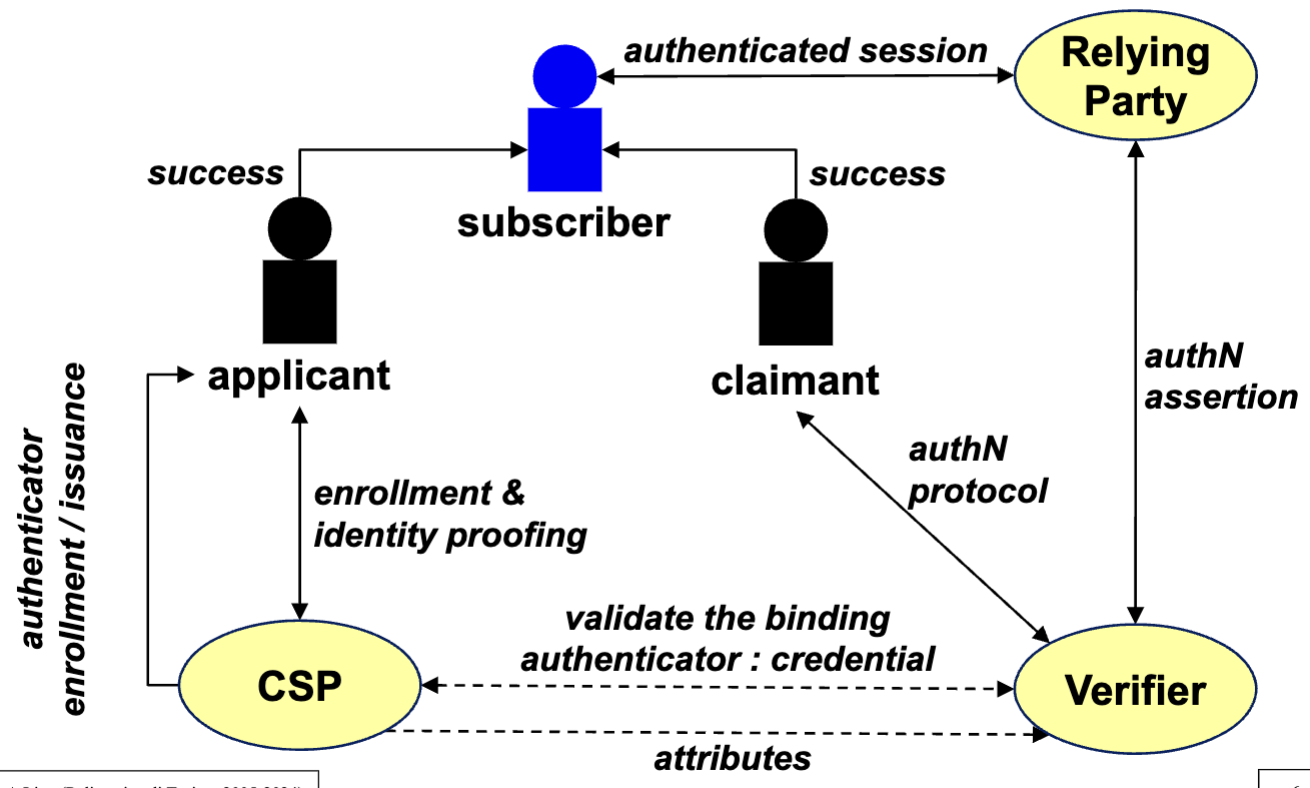
\includegraphics[width=0.6\linewidth]{Images/Authentication/auth_model.png}
    \caption{Digital Authentication Model}
\end{figure}

\begin{tcolorbox}[colback=blue!10!white, colframe=blue!50!white]
Credential binds an authenticator to the subscriber's identity (e.g., X.509 certificate).
\end{tcolorbox}

\section{Generic Authentication Protocol}
\begin{enumerate}
    \item The verifier sends an authentication request to the user (claimant).
    \item The user sends his ID to the verifier.
    \item The verifier checks the ID against the stored credential data. Then, it sends a proof request (“Is this really you?”) to the user.
    \item The user sends an authentication response by submitting the appropriate authenticator $f(S_{UID})$\footnote{f may be a hash function.} (e.g., password, OTP, fingerprint) (Better if the channel is secure).
    \item The verifier checks the submitted response against the stored credential data (Mapped as UID:f($S_{UID}$)).
\end{enumerate}

\begin{figure}[H]
    \centering
    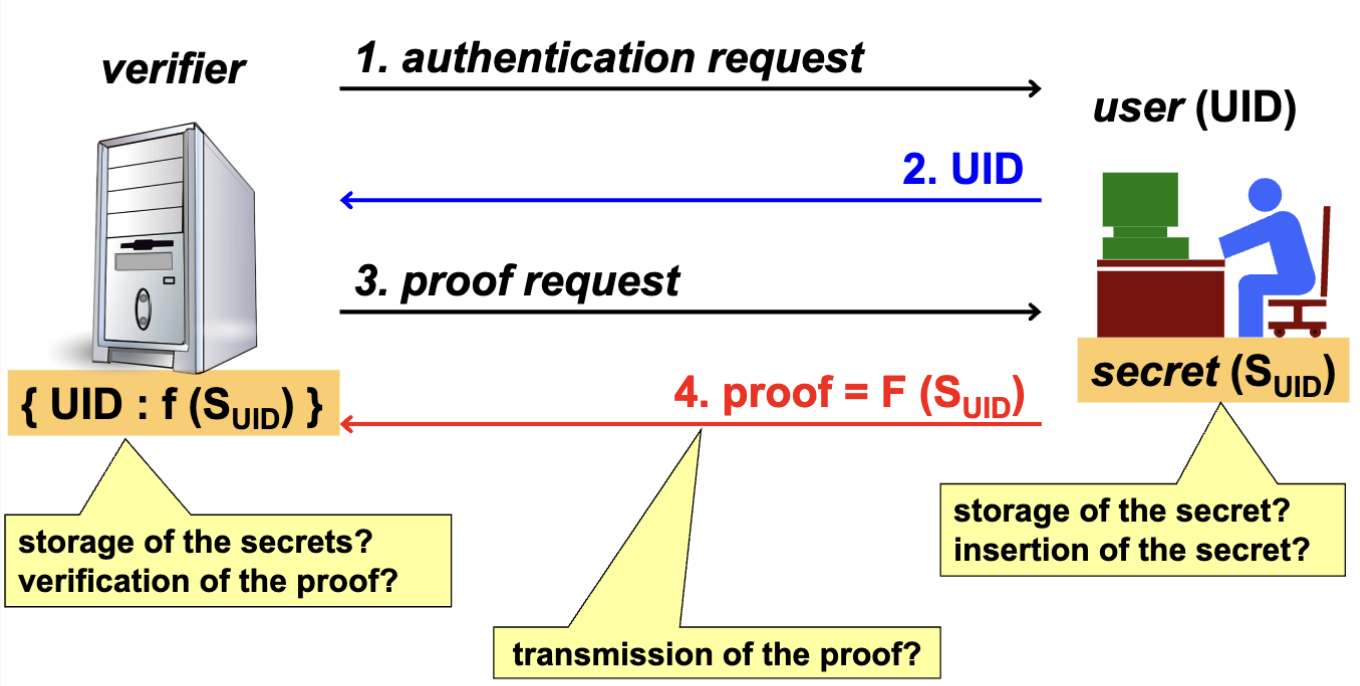
\includegraphics[width=0.5\linewidth]{Images/Authentication/authNprot.png}
    \caption{Generic Authentication Protocol}
\end{figure}

\subsection{Password-based Authentication}
The user's secret is the password. 

The verifier may have stored the password:
\begin{itemize}
    \item In cleartext.
    \item One-way hashed.
\end{itemize}
In order to verify the proof given by the user, the verifier must either check if the password is the same as the one stored or hash the password and compare the digest with the stored hash.

\begin{tcolorbox}[colback=red!10!white, colframe=red!70!black, coltitle=white, title=Beware]
Even if the password is hashed, it is still vulnerable. For example, the attacker can use a dictionary attack or a brute-force attack.
\end{tcolorbox}
\begin{figure}[H]
    \centering
    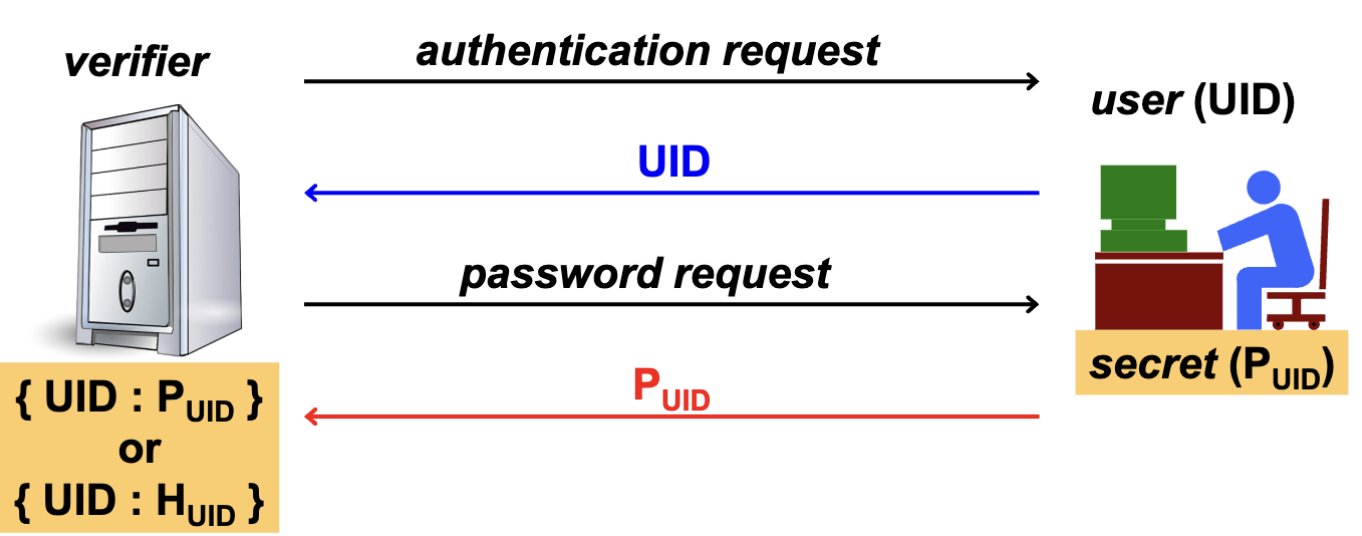
\includegraphics[width=0.5\linewidth]{Images/Authentication/pb_authn.png}
    \caption{Password-based Authentication}
\end{figure}



\clearpage
\begin{multicols}{2}
    \center{\subsubsection*{Reusable Passwords}}
    Reusing passwords can be dangerous:
    \begin{itemize}
        \item Password sniffing.
        \item Password DB attacks.
        \item Password guessing.
        \item Password enumeration (brute force attack): This occurs in the case of length-constrained passwords (or when fewer subsets of characters are available), or when the authentication protocol does not block multiple attempts.
        \item Password duplication: The same password is used for different services.
        \item Cryptography aging: In future years, cryptographic algorithms may become weak due also to the increasing computational power.
        \item Password capture (via spoofing or phishing).
        \item MITM attacks.
    \end{itemize}
    \columnbreak

    \center{\subsubsection*{Best Practices}}
    \begin{itemize}
        \item Alphabetic characters (upper and lower case) + digits + special characters.
        \item Must be at least 8 characters long (Brute force attack).
        \item Never use dictionary words.
        \item Frequently changed (but not too frequently).
        \[ \text{Password Age } \Delta t \le T_A =  {\text{items}^{\text{length}} \over 2}  \]
        \item Find alternative authentication methods (e.g., biometrics).
    \end{itemize}
    
\end{multicols}

\subsection*{Password Storage}
\begin{multicols}{2}
    Server-side password storage:
    \begin{itemize}
        \item NEVER in cleartext.
        \item Digest of the password (Dictionary attack, also with Rainbow Table).
        \item "Salted" hash: $H(Salt || Password)$.
    \end{itemize}
    
    \columnbreak

    Client-side password storage:
    \begin{itemize}
        \item Should be only in the user's end ... but too many passwords.
        \item Use an encrypted file or a password wallet/manager.
    \end{itemize}
\end{multicols}

\begin{tcolorbox}[colback=blue!10!white, colframe=blue!50!white]
For Dictionary Attack and Rainbow Table, the attacker can use a precomputed table of hashes for all possible passwords. See Appendix A for more information.
\end{tcolorbox}

\subsection{Password Salting}
\begin{center}
    The only correct way to store passwords.\\ \textcolor{Blue}{Does not admit dictionary attacks or those based on rainbow tables(pre-computation attacks).}
\end{center}
How it works, for each user ID (UID):
\begin{itemize}
    \item Create/ask the password.
    \item Generate a salt (different for each UID): A random (unpredictable) and long enough string, which should contain rarely used or control characters.
    \item Compute the Salted Hash of Password \(SHP = H(Salt || Password)\).
    \[\text{The salt is concatenated with the password.} \]
    \item Store (server/client-side) the triples \((\text{UID, Salt, SHP})\).
\end{itemize}
Additional benefit: we have different SHP for users having the same password !

\vspace{0.3cm}

\begin{center}
    \textbf{Using the salted password in the authentication protocol:}
\end{center}
\begin{verbatim}
    Claimant > Verifier: (UID, pwd)

    Verifier:
        1. Checks if the UID is in the DB.
            1a. If not, abort: "AuthN Failure".
            1b. If yes, retrieves Salt and SHP.
        2. Computes SHP' = H(Salt || pwd).
        3. Compares SHP' with SHP.
            3a. If not equal, "AuthN Failure".
            3b. If equal, "AuthN Success".
\end{verbatim}

\begin{tcolorbox}[colback=red!10!white, colframe=red!70!black, coltitle=white, title=Beware]
Never give information about authentication failures. This could help attackers to guess the password.
\end{tcolorbox}

\subsection*{Passwords in Linux}
Originally stored in \texttt{/etc/passwd} (readable by everyone) hashed with a DES-based hash function named \texttt{crypt()}. Now stored in \texttt{/etc/shadow} (readable only by root).

\vspace{0.2cm}

Passwords are stored in the form:
\begin{itemize}
    \item \texttt{username:\$uid\$salt\$hashedpwd ...}
    \item Are used different hash functions depending on ID, for example:
    \begin{itemize}
        \item 1: MD5.
        \item 5: SHA-256.
        \item 6: SHA-512.
        \item y: YesCrypt.
    \end{itemize}
    \item If \texttt{\$uid\$salt} is absent then the old DES-based hash is used, with 12-bit salt, pwd truncated to 8 characters \textcolor{Red}{(not secure!!)}.
\end{itemize}

If you want to try yourself, you can use:
\begin{lstlisting}[style=bashStyle]
# gain root access
sudo su
# add user w/o pwd
sudo adduser test1 --disabled-password
# create pwd string with selected hash algo and salt
mkpasswd --method=md5 --salt=coolsalt 1234

# view the hash of 1234
echo -n 1234 | openssl dgst -md5
# in the /etc/shadow file you would see: 
#       $1$coolsalt$qTXiZzGn08J.xYkV1ce1y1:...
#   IDK the manual-hashed password don't correspond to the one given by mkpasswd ... correct me if I'm wrong
\end{lstlisting}

\subsection*{Passwords in MySQL}
Username and password are stored in the \texttt{mysql.user} table. MySQL (from v4.1) uses a double hash (\textcolor{Red}{not salted!!}) to store the password.
\[SHA1(SHA1(password)) \qquad \text{Very Poor Solution...}\]
\begin{lstlisting}[style=bashStyle]
# perform the double (but different) hash on the password
echo -n 'password' | openssl sha1 -binary | openssl sha1 -hex
# the stored output is: 2470c0c06dee42fd1618bb99005adca2ec9d1e19

\end{lstlisting}

\section{Strong (Peer) Authentication}
"Strong Authentication" is often requested in many specifications, but has never been defined in a standard way. It is often used to indicate that the authentication process is based on more than one factor.

\subsection*{ECB Definition}
\begin{center}
    (European Central Bank Definition)
\end{center}
Some elements of the ECB definition:
\begin{itemize}
    \item Strong customer authentication is a procedure based on the use of two or more of knowledge, ownership, and inherence. 
    \item The elements selected must be mutually independent (the breach of one does not compromise the others).
    \item At least one element should be non-reusable and non-replicable (except for inherence), and not capable of being surreptitiously stolen via the internet.
    \item The strong authentication procedure should be designed in such a way as to protect the confidentiality of the authentication data.
\end{itemize}

\subsection*{PCI-DSS Definition}
\begin{center}
    (Payment Card Industry Data Security Standard Definition)
\end{center}
PCI-DSS requires strong authentication for access to Cardholder Data Environment (CDE). It is defined for:
\begin{itemize}
    \item Remote access from trusted or untrusted networks.
    \item By users, third-parties (e.g. maintenance) and administrators.
    \item Exception: direct console access (physical security).
\end{itemize}
Compulsory after 2018.
\begin{tcolorbox}[colback=red!10!white, colframe=red!70!black, coltitle=white, title=Beware]
Multi-factor authentication is NOT twice the same factor (e.g., two passwords).
\end{tcolorbox}

\subsection*{Other Definitions}
Strong authentication as:

\vspace{0.3cm}

\blockquote[Handbook of Applied Cryptography]{A cryptographic challenge-response identification protocol.}

\vspace{0.3cm}

\noindent More in general:

\blockquote{Technique resisting to a well-defined set of attacks.}

\vspace{0.3cm}


In conclusion, an authentication (authN) technique can be regarded as strong or weak depending on the \textbf{attack model}. For example, users of Internet banking services would probably prefer the ECB definition, while employees of PSP (Payment Service Providers) would prefer the PCI-DSS definition.

\begin{tcolorbox}[colback=blue!10!white, colframe=blue!50!white]
Watch out for you specific application field (risks and threats in that environment).
\end{tcolorbox}

\section{Challenge-Response Authentication}
\begin{center}
    CRA - General Model
\end{center}


\begin{multicols}{2}
\begin{itemize}
    \item The claimant tries to enter a system with his User ID.
    \item The verifier sends a challenge to the claimant.
    \item The claimant replies with the solution computed using some secret knowledge and the challenge.
    \item The verifier compares the response with a solution computed  via a secret associated to the claimant.
\end{itemize}

\columnbreak

    \begin{figure}[H]
        \centering
        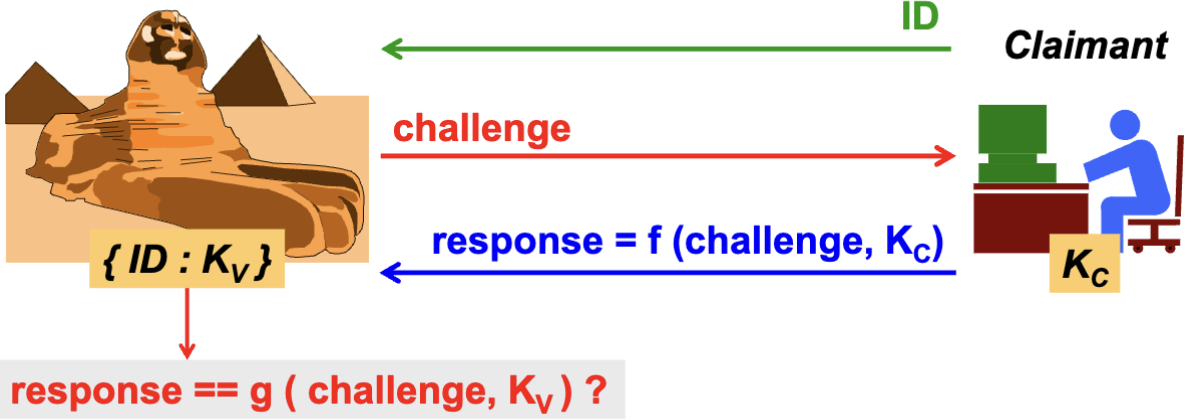
\includegraphics[width=\linewidth]{Images/Authentication/CRA.png}
        \caption{Challenge-Response Authentication model}
    \end{figure}
\end{multicols}

\subsection*{CRA - General Issues}
\begin{itemize}
    \item The challenge must be non-repeatable to avoid replay attacks. Usually the challenge is a (random) nonce.
    \item The function $f$ must be non-invertible (one-way function) otherwise, a listener can record the traffic and easily find the shared secret.
    \[
        if(\nexists f^{-1}) \text{ then } K_C = f^{-1} (response, challenge)
    \]
\end{itemize}

\subsection{Symmetric CRA}
Claimant and Verifier share a secret key \(K_{ID}\) (e.g., a password or a key).


\begin{multicols}{2}

    \begin{itemize}
        \item A challenge is sent to the claimant.
        \item The claimant computes the response as \(response = f(K_{ID}, challenge)\). Then sends it to the verifier.
        \item The verifier computes the expected response as \(response' = f(K_{ID}, challenge)\) and compares it with the received response.
    \end{itemize}
    
\columnbreak

    \begin{figure}[H]
        \centering
        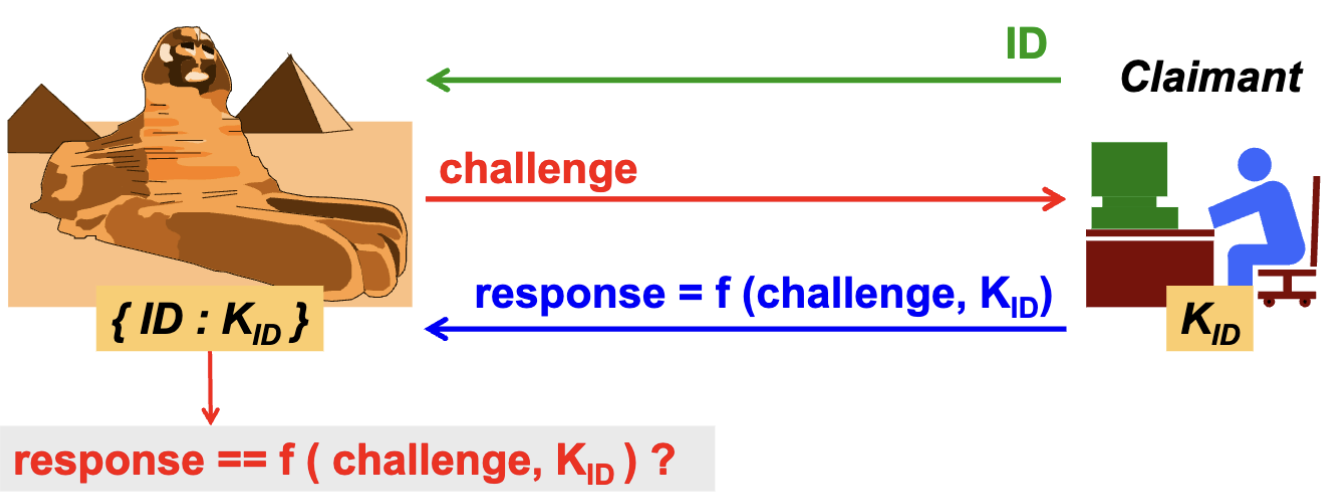
\includegraphics[width=\linewidth]{Images/Authentication/symCRA.png}
        \caption{Symmetric Challenge-Response Authentication}
    \end{figure}
\end{multicols}

\subsection*{Symmetric CRA - General Issues}
The easiest implementation uses a hash function (e.g. SHA1, deprecated). $K_{ID}$ must be known in cleartext to the verifier (possible attacks). SCRAM (Salted Challenge Response Authentication Mechanism) is a better solution, by using hashed passwords at the Verifier side (offers also secure channel binding and mutual authentication).

\clearpage
\subsection{Mutual Symmetric Challenge-Response Authentication} 
\begin{center}
    General exchange - Deprecated.\\
    Both parties authenticate each other using a shared \\secret key and challenge-response mechanisms.\\ 
\end{center}
\begin{tcolorbox}[colback=red!10!white, colframe=red!70!black, coltitle=white, title=Beware]
The protocol (and so its related problem) relies on demonstrating the knowledge of the shared secret.
\end{tcolorbox}

\begin{multicols}{2}

    \begin{center}
        {\large{\textbf{v1:}}}
    \end{center}
    \begin{itemize}
        \item Only the initiator (of the communication) provides explicitly its (claimed) identity.
    \end{itemize}
    \begin{figure}[H]
        \centering
        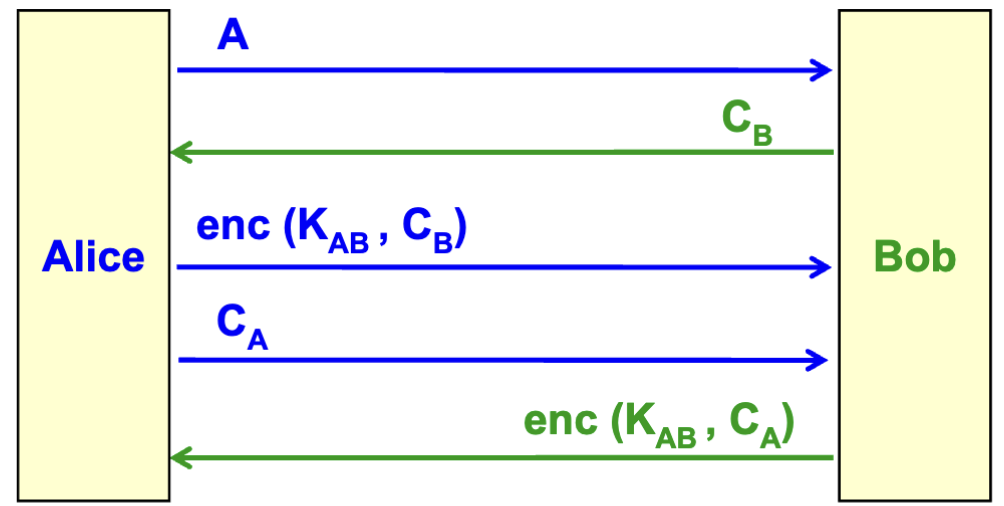
\includegraphics[width=\linewidth]{Images/Authentication/msCRA.png}
        \caption{Mutual Symmetric Challenge-Response Authentication first version}
    \end{figure}
    \columnbreak

    \begin{center}
        \large{\textbf{v2:}}
    \end{center}
    \begin{itemize}
        \item Only the initiator (of the communication) provides explicitly its (claimed) identity.
        \item Fewer messages.
        \item Better performance, but still no impact on security.
    \end{itemize}

    \begin{figure}[H]
        \centering
        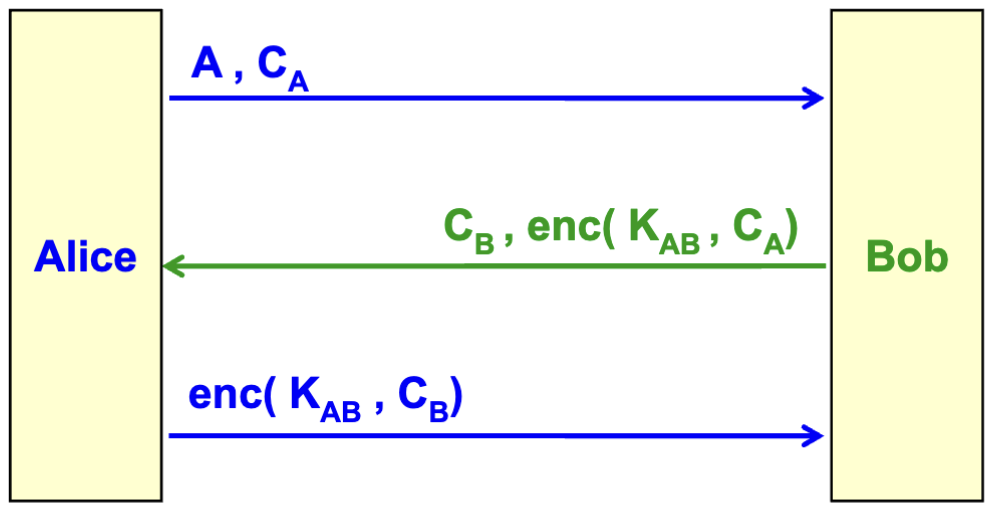
\includegraphics[width=\linewidth]{Images/Authentication/msCRAv2.png}
        \caption{Mutual Symmetric Challenge-Response Authentication second version}
    \end{figure}
    
\end{multicols}

\subsubsection*{Mutual Symmetric CRA - Process}
\begin{center}
    v1:
\end{center}
Alice to Bob authentication:
\begin{itemize}
    \item The initiator (Alice) sends her ID to the responder (Bob).
    \item Bob sends a challenge to Alice.
    \item Alice encrypts the challenge with her secret key and sends it to Bob.
    \item Bob decrypts the response and checks if it is correct.
\end{itemize}
\dots\ Bob to Alice authentication:
\begin{itemize}
    \item Alice sends a challenge to Bob.
    \item Bob encrypts the challenge with his secret key and sends it to Alice.
    \item Alice decrypts the response and checks if it is correct.
\end{itemize}

\subsection*{Mutual Symmetric CRA - Attack}
\begin{center}
    Exploits the fact that the same key is used for both directions.
\end{center}




\begin{multicols}{2}

    \begin{itemize}
        \item Mike (the attacker pretending to be Alice) creates a first connection by sending Alice's identifier $A$ along with a random challenge $C_A$ to Bob.
        \item Bob replies with the encrypted challenge-response and a new challenge $C_B$ (due to mutual authentication).
        \item Mike stores the new challenge, then\dots
    \end{itemize}
    \columnbreak

    \begin{figure}[H]
        \centering
        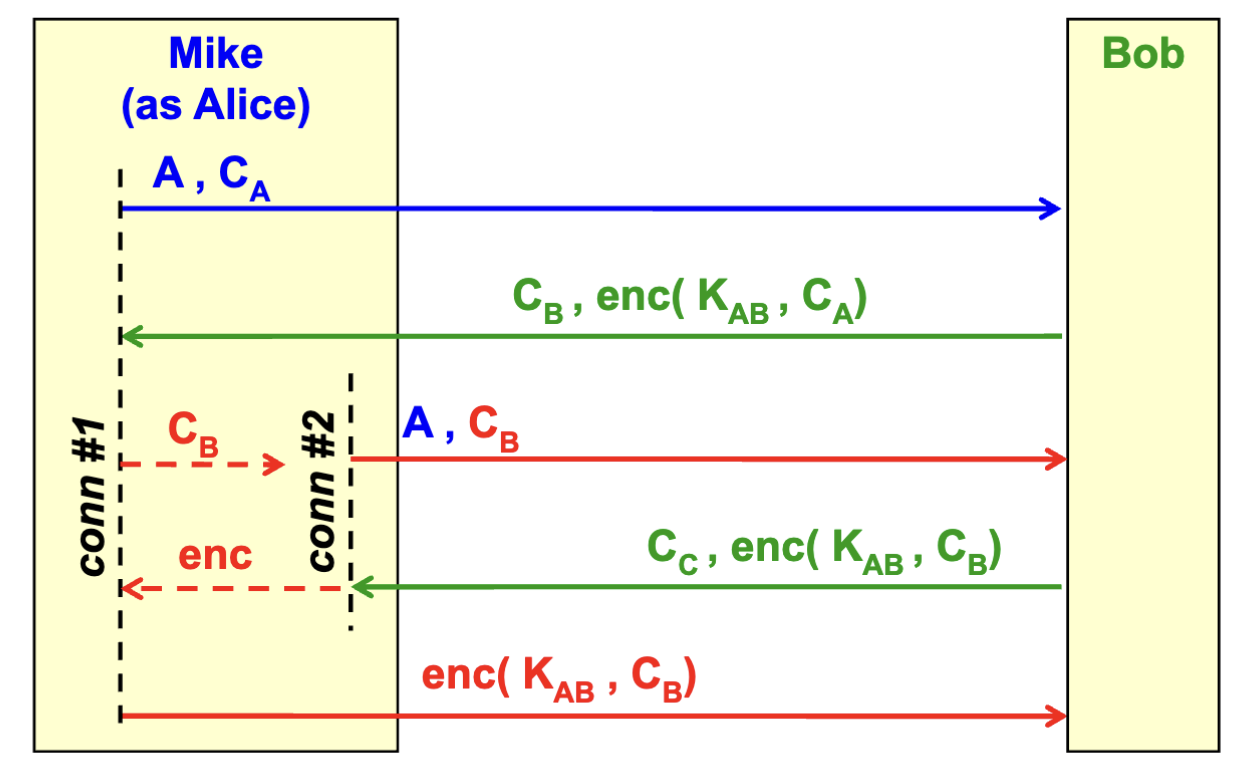
\includegraphics[width=\linewidth]{Images/Authentication/msCRAatt.png}
        \caption{Attack to Mutual Symmetric CRA}
    \end{figure}
\end{multicols}
\begin{itemize}
    \item Mike creates a second connection by sending Alice's identifier $A$ and replaying ($\ne$ replying) the challenge $C_B$, which was received earlier from Bob.
    \item Bob replies with the encrypted challenge $C_B$(the previous one sent by Bob) and a new challenge $C_C$.
\end{itemize}

\subsubsection{Global System for Mobile Communications (in)Security}
\begin{center}
    GSM insecurity.
\end{center}
GSM uses three secret algorithms:
\begin{itemize}
    \item $A8$ for symmetric key generation (in the SIM).
    \item $A3$ for authentication (in the SIM).
    \item $A5$ (stream cipher) for encryption (in the mobile device).
\end{itemize}
This is security-through-obscurity \dots always a bad idea !
The three algorithms above are left to the choice of the MNO (Mobile Network Operator) and are not standardized.
\begin{tcolorbox}[colback=blue!10!white, colframe=blue!50!white]
$A8$ and $A3$ are usually built upon the COMP128 (secret) function.
\end{tcolorbox}

\clearpage
\subsubsection*{GSM Authentication Mechanism}
\begin{multicols}{2}

    The authentication protocol uses a symmetric challenge-response mechanism to authenticate the Mobile Station (MS) via its SIM card to the Base Station (BS). The process works as follows:
\columnbreak

    \begin{figure}[H]
        \centering
        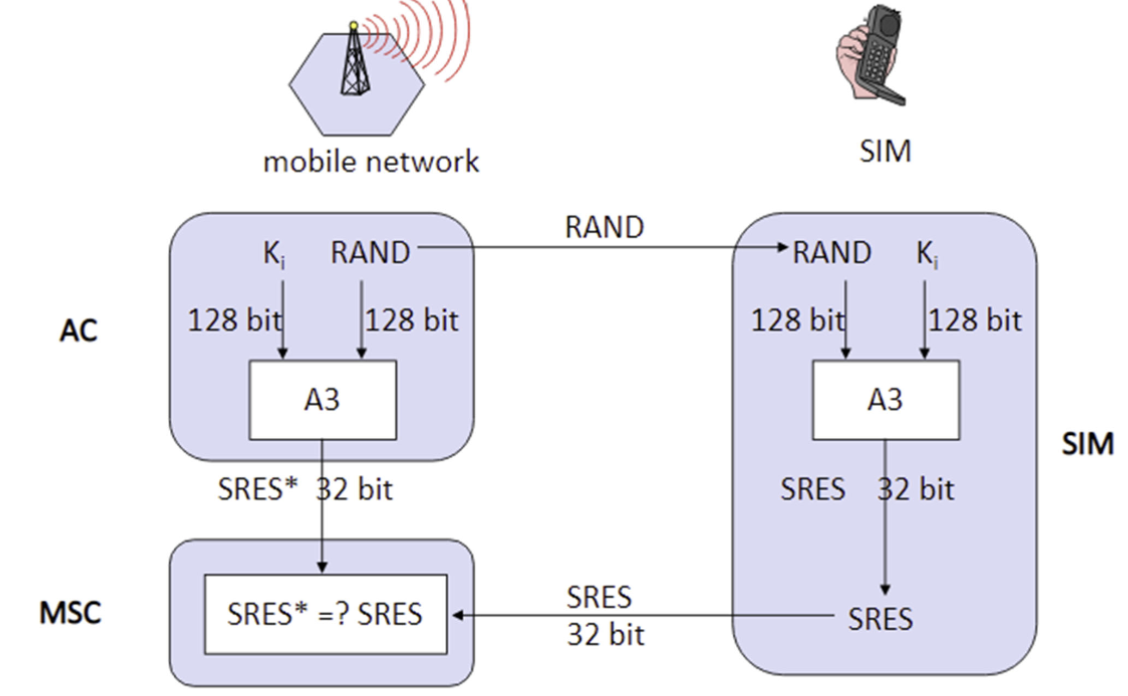
\includegraphics[width=\linewidth]{Images/Authentication/gsm_authn.png}
        \caption{GSM Authentication Mechanism}
    \end{figure}
\end{multicols}

\begin{itemize}
    \item The BS sends to the SIM card a random challenge $C$ of 128 bits. 
    
    \hspace*{1cm} This challenge is intended to verify the possession of \\ \hspace*{3cm} the shared secret key  $K_i$  stored securely on the SIM.
    \item The SIM computes the response as $SRES = A3(K_{i}, C)$ of 32 bits.
    \begin{itemize}
        \item COMP128-1 is weak \dots with chosen-challenge (and differential cryptanalysis) $150k$ challenges are enough to compute the secret key $K_i$.
        \item \dots\ then an attacker could clone the SIM card and \\\hspace*{4cm} decrypt the traffic by computing $K_c$.
        
        $K_c$  is a session key established between the Mobile Station (MS) and the Base Station (BS), and it is derived from the secret key  $K_i$  (stored on the SIM card) and the random challenge $C$  sent by the BS.
    \end{itemize}
\end{itemize}

\subsection{Asymmetric CRA}
Claimant and Verifier have different secret keys. Both entities have a pair of keys: a public key and a private key. The public key is known to everyone, while the private key is known only to the owner.

\begin{multicols}{2}

    \begin{itemize}
        \item The Claimant sends his public-key certificate to the Verifier.
        
        The certificate contains the public key $ID.PK$ and the claimant's ID.
        \item The verifier encrypts a random nonce $R$ with the claimant's public key $ID.PK$ (asymm. encryption) and sends it to the claimant.
        \item The claimant decrypts the nonce with his private key $ID.SK$ and sends it back to the verifier.
    \end{itemize}

    \columnbreak
\begin{figure}[H]
    \centering
    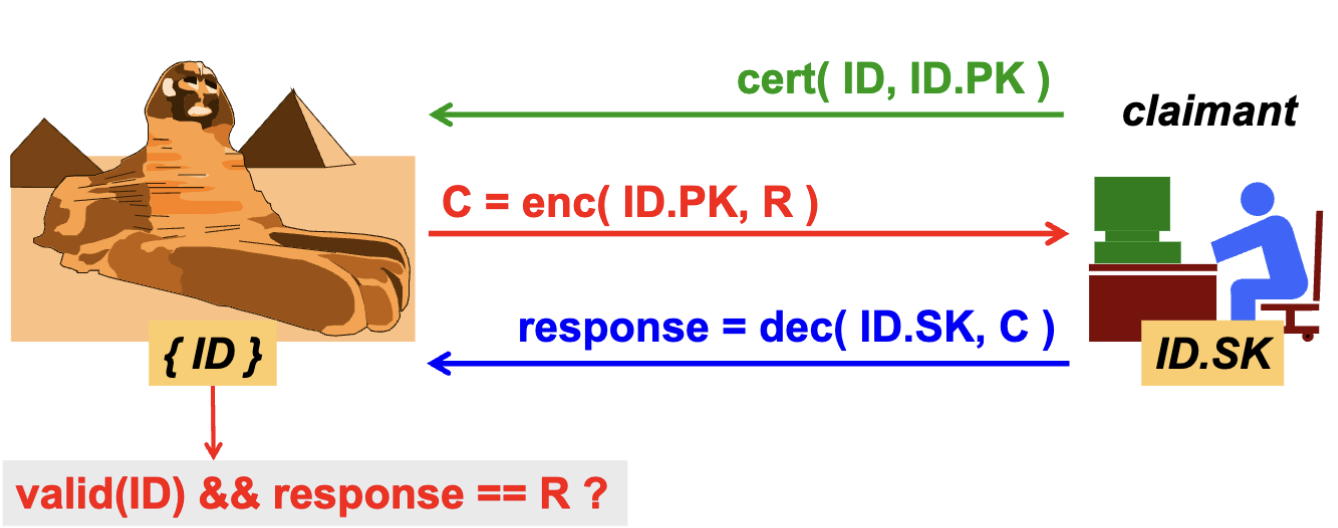
\includegraphics[width=\linewidth]{Images/Authentication/asymmCRA.png}
    \caption{Asymmetric Challenge-Response Authentication}
\end{figure}

\end{multicols}

At the end, the Verifier checks if the received nonce is the same as the one sent. The claimant has demonstrated the possession of the private key associated with the public key in the certificate.

\subsection*{Asymmetric CRA - Analysis}
\begin{itemize}
    \item The strongest mechanism.
    \item Does not require secret storage at the Verifier side.
    \item Applications: Implemented for peer authentication (client and server) in IPsec, SSH, TLS.
    \item Cornerstone for user authentication in FIDO (Fast Identity Online).
\end{itemize}
\subsection*{Asymmetric CRA - General Issues}
\begin{itemize}
    \item Slow.
    \item If designed inaccurately may lead to an involuntary disclosure of the private key.
    \item PKI (Public Key Infrastructure) issues (trusted root, name constraint, revocation, etc.).
    
    This could be avoidable if the Verifier stores $ID.PK$ in a secure way \dots \ but this moves equivalent PKI effort to the Verifier.
\end{itemize}

\section{One-Time Password}
\begin{center}
    OTP - General Model
\end{center}
\begin{multicols}{2}

    \begin{itemize}
        \item The verifier sends an authentication request to the user.
        \item The user sends his ID to the verifier.
        \item The verifier requests a one-time password (OTP) to the user (no.48 in the figure's case).
        \item The server computes the expected value of P48 in real-time using the shared secret $S_{UID}$, the counter, and a function $p$.
        
        \begin{itemize}
            \item The function $p$ is a \textbf{keyed-digest} (key+data/counter) function (e.g., HMAC-SHA1).
        \end{itemize} 
    \end{itemize}

    \columnbreak

    \begin{figure}[H]
        \centering
        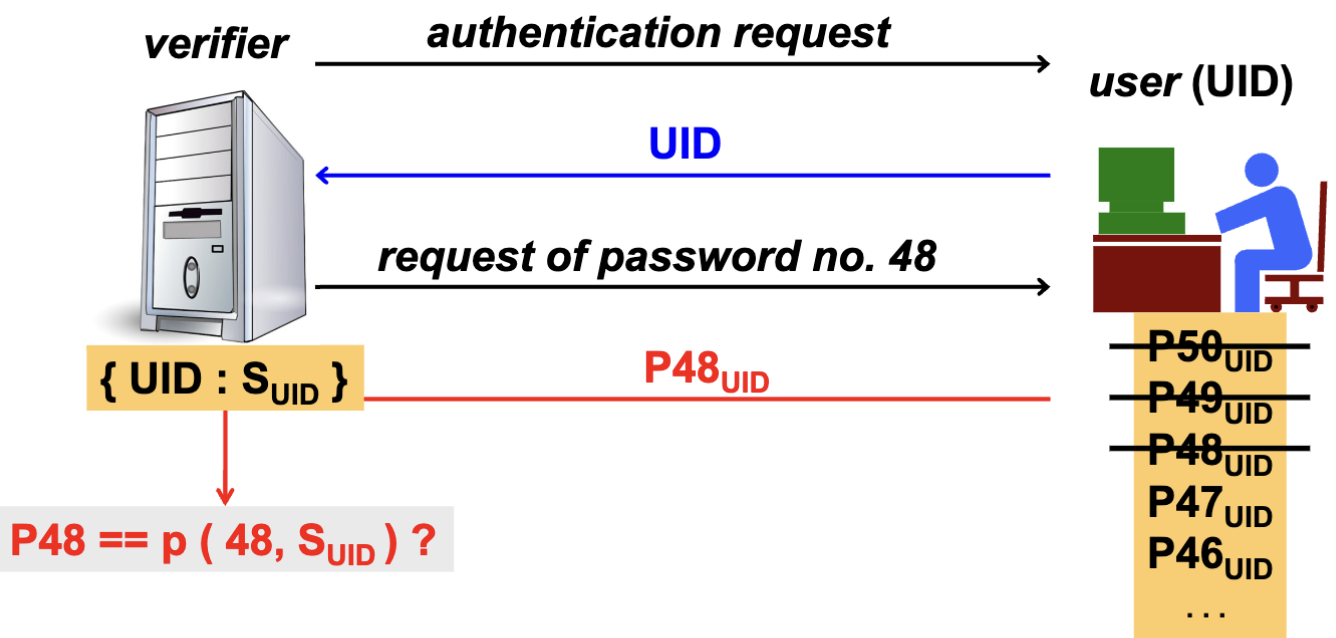
\includegraphics[width=\linewidth]{Images/Authentication/OTP.png}
        \caption{One-Time Password}
    \end{figure}
    
\end{multicols}
If the provided password  $P48_{UID}$  matches the server’s computed value  $p(48, S_{\text{UID}})$, the user is authenticated successfully.

\subsection*{OTP - Analysis}
\begin{itemize}
    \item The password is valid only for one run of the authentication protocol (Next run requires a new password).
    \item Immune to sniffing.
    \item Subject to MITM (needs Verifier to be authenticated).
    \item Difficult provisioning to the subscribers/users: Lots of passwords to remember, password exhaustion (time limit for use).
    \item Difficult password insertion: Verbose and mixed (Contains random characters to avoid guessing attacks) on purpose.
\end{itemize}

\subsection*{OTP - Provisioning to Users}
On naive systems, or insecure/untrusted workstation:
\begin{itemize}
    \item Paper sheet of precomputed passwords ("password cards").
    \item Hardware authenticators ("crypto tokens")(e.g., RSA SecurID or Google authenticator).
\end{itemize}
On intelligent and secure/trusted workstation:
\begin{itemize}
    \item Automatically computed by an ad-hoc application.
    \item Typically, the OTP is generated by a smartphone app.
\end{itemize}

\subsection{The Secure Key System}
\begin{center}
    S/KEY System for Off-line/Precomputed One-Time Passwords.
\end{center}

First OTP definition and implementation by Bell Labs (1981). 
\begin{itemize}
    \item The user generates a secret $S_{ID}$ and a sequence of OTPs.
    \[
        \begin{aligned}
            &P_1 = h(S_{ID}) \\
            &P_2 = h(P_1) \\
            &\dots \\
            &P_n = h(P_{n-1})\\\\
            \text{h is a } &\text{hash } \text{function (e.g. md4).}
        \end{aligned}
    \]
    \item The Verifier stores the last one OTP used $P_n$: This password will never be used directly for authentication.
    \item Verifier requests $P_{n-1}$, and receives $X$ (reverse order of requests).
    \[
        P_n \ne h(X)\quad ?\quad \text{"OK, store X as } P_{n-1}\text{"} : \text{"AuthN Failure"}
    \]
    In this way the Verifier has no need to know the user's secret and only the user knows all passwords.
\end{itemize}

\begin{figure}[H]
    \centering
    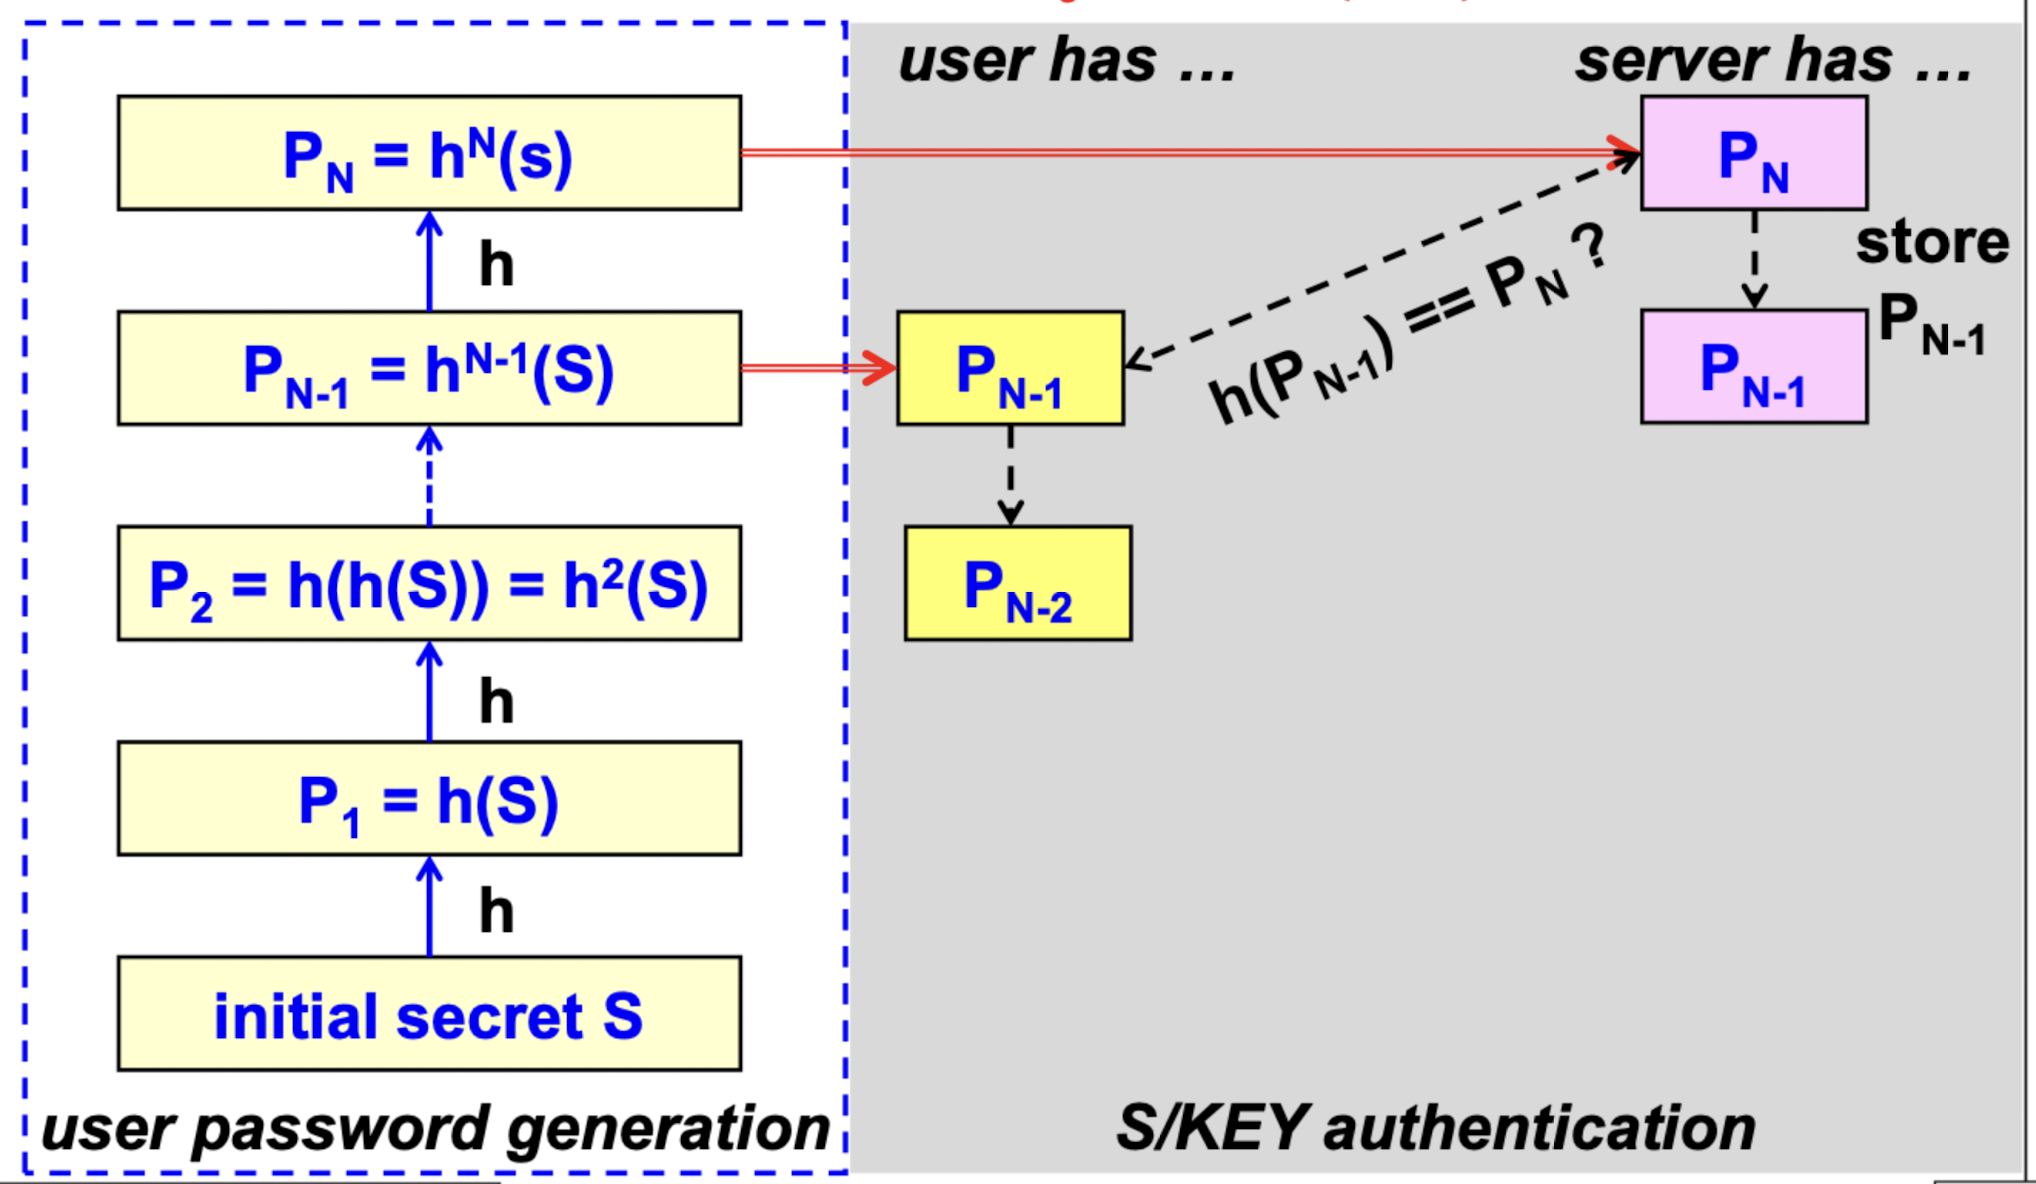
\includegraphics[width=0.5\linewidth]{Images/Authentication/skey.png}
    \caption{Secure Key System Model}
\end{figure}

\subsubsection*{S/KEY - Password-Chain Generation}
\begin{center}
    The real implementation uses a seed and a pass phrase.
\end{center}
\begin{enumerate}
    \item The user generates a Pass Phrase (PP) $S_{ID}$: Minimum 8 characters long, mixed, and secret! (if exposed the security of S/KEY is compromised).
    \item PP is concatenated with a server-provided seed 
    
    The seed is not secret; it is sent in cleartext from the server to the client. It allows the reuse of a passphrase (PP) (using different seeds).
    \item A 64-bit quantity is extracted from the $md4(PP||seed)$ hash (output of 128-bit).
    
    This is achieved by XORing the first 32-bit group with the third 32-bit group, and the second 32-bit group with the fourth 32-bit group.
\end{enumerate}

\subsubsection*{S/KEY - Passwords}
\begin{itemize}
    \item 64-bit passwords are a compromise:\\\hspace*{3cm}Neither too long (complex) nor too short (easy to guess).
    \item Entered as a sequence of 6 short English words\footnote{Instead of just random bits, to make them easier for users to remember.} chosen from a dictionary of 2048 \\(e.g. 0="A", 1="ABE", 2="ACE", 3="ACT", 4="AD", 5="ADA")
    
    \dots Client and Server must share the same dictionary.
    \\\hspace*{1cm} e.g. text-password: "YOU SING A NICE OLD SONG"
    \\\hspace*{1cm} e.g. numeric-password (hex): "1D6E5001884BD711"
\end{itemize}
\subsection{Time-Based One-Time Password}
\begin{center}
    TOTP - General Model.
\end{center}
The password depends upon time (e.g. valid for 30 seconds) and the User-Verifier shared secret.
\[
    \boxed{p(K_{ID}, t)=h(S_{ID}, t)}
\]
$h$ : A cryptographic hash or HMAC (better) function used to generate the token.\\
$t$: The current time (e.g., in seconds or milliseconds).
\begin{multicols}{2}

    \begin{itemize}
        \item The Verifier sends an authentication request to the user.
        \item The Claimant sends his $ID$ and $X$ ($=p(text{ID}, t)$) to the Verifier. 
        \item The Verifier also computes $X$, but using the stored information, and compares it with the received one.
    \end{itemize}
\columnbreak

    \begin{figure}[H]
        \centering
        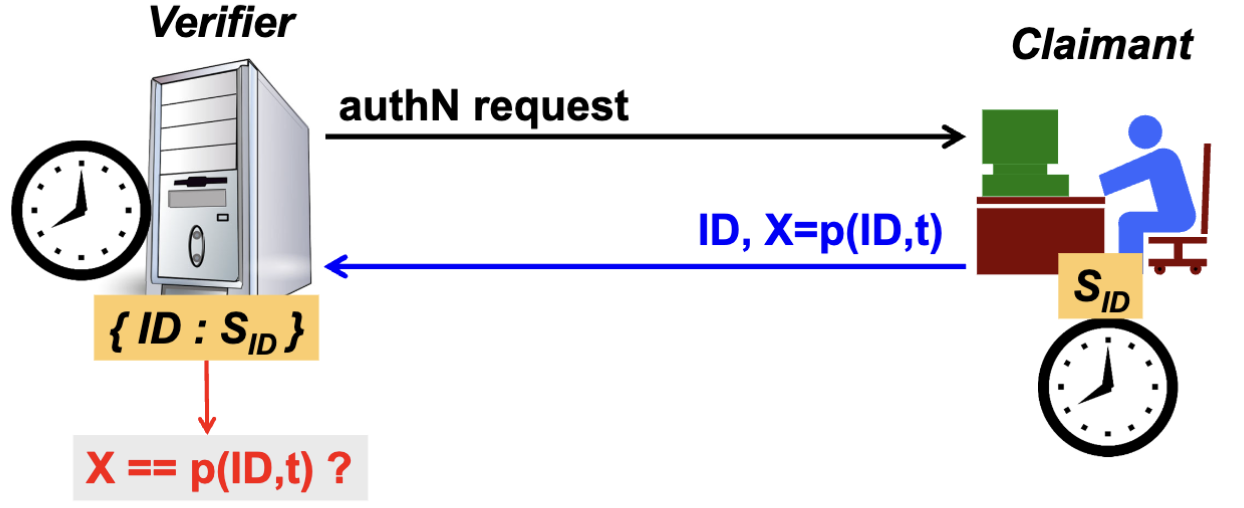
\includegraphics[width=\linewidth]{Images/Authentication/totp.png}
        \caption{Time-Based One-Time Password}
    \end{figure}
\end{multicols}

\subsection*{Time-Based OTP - Analysis}
\begin{itemize}
    \item Requires local computation at the subscriber/claimant side.
    \item Requires clock synchronization or keeping track of time-shift for each subscriber.
    
    Desynchronization can be a cause to DDoS attacks or passwords stealing.
    \item Requires time-slot and authentication window management.
    
    Tolerance window for time-based authentication:
    \\\hspace*{1cm}(It ensures flexibility when verifying the validity of a time-based proof or token  X)
    \[
        X==p(text{ID}, t) \quad \| \quad X == p(text{ID}, t-1) \quad \| \quad X == p(text{ID}, t+1)
    \]
    \item Only one authentication run per time-slot (typically 30 seconds or 60s).
    \item Time attacks against subscribers and Verifier: For example, fake NTP (Network Time Protocol) server.
    \item Sensitive database at the Verifier side  (e.g. attack against RSA SecurID).
\end{itemize}
\begin{tcolorbox}[colback=blue!10!white, colframe=blue!50!white]
Antennas can be used to synchronize the clocks of the devices.
\end{tcolorbox}

\subsubsection*{Time-Based OTP - RSA SecurID}
\begin{center}
    A concrete implementation of TOTP (Time-Based OTP).
\end{center}
\begin{itemize}
    \item The Claimant sends to the Verifier in clear: user, PIN, token-code (seed + current time). The token-code can comprehend the PIN also (if an authenticator with pinpad is used).
    \item Based on user and PIN the Verifier checks the token-code sent by the claimant against three possible time windows to account for clock drift:
    \begin{itemize}
        \item  $TC_{-1}$ : Token-code from the previous time window.
        \item $TC_0$ : Token-code from the current time window.
        \item $TC_{+1}$ : Token-code from the next time window.
    \end{itemize}
    \item "Duress Code": A special code that can be used to authenticate the user in case of coercion (apparently does the same as the normal code, but it triggers an alarm).
\end{itemize}
\subsubsection*{RSA SecurID - Architecture}

The RSA SecurID system is composed of:
\begin{itemize}
    \item Claimant: The user who wants to authenticate.
    \item ACE Client: Installed on the Relying Party. Establishes the connection with the subscriber and forwards authentication information to the ACE server for verification.
    \item ACE Server: The core authentication verifier. Checks the validity of the SecurID token code, user credentials (PIN, etc.).
\end{itemize}
Left side of the figure \ref{fig:secarch} is a successful authentication, right side is a failed authentication.

\begin{figure}[H]
    \centering
    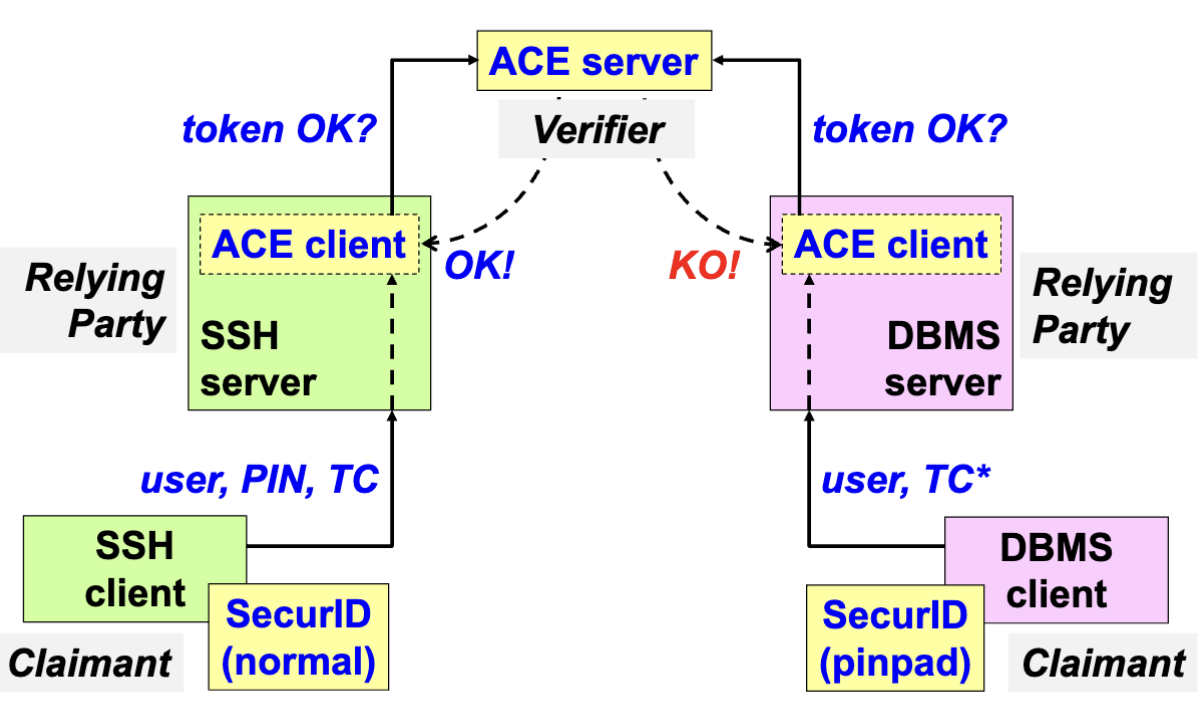
\includegraphics[width=0.5\linewidth]{Images/Authentication/secarch.png}
    \caption{RSA SecurID Architecture}
    \label{fig:secarch}
\end{figure}

\subsection{Event-Based One-Time Password}
\begin{center}
    Event-Based OTP - General Model.
\end{center}
The password depends upon the event (e.g. a button press) and the User-Verifier shared secret.
\begin{itemize}
    \item Uses monotonic integer counter $C$ as input besides the seed.
    \[
        p(\text{ID}, C)=h(S_{ID}, C) \quad \text{with } C \in \mathbb{Z} \land\text { monotonic}
    \]
    \item Requires local computetion at the subscriber/claimant side.
    \item Frequent authentication runs are possible.
    \item Because the counter is event-driven, the user can generate OTPs frequently without waiting for time slots (unlike time-based OTPs).
    \item OTPs can be generated in advance because they depend only on the counter value and the seed:
    \begin{itemize}
        \item Useful for travel: Users can carry pre-computed OTPs to avoid losing access (e.g., when they don’t have their token).
        \item Security Risk: An adversary with temporary access to the authenticator can pre-compute OTPs, increasing the risk of misuse.
    \end{itemize}
    \item The counter on the user’s device (subscriber) may become out of sync with the verifier (e.g. manual increments) so, the verifier must accommodate desynchronization by checking a range of counter values:
    \[
X == p(\text{ID}, C) \, \| \, X == p(\text{ID}, C+1) \, \| \, X == p(\text{ID},C+2) \, \| \, \dots
    \]
    How big should be the tolerance window? It depends on the application and the risk of desynchronization.
\end{itemize}

\subsection{Out-of-Band One-Time Password}
\begin{center}
    Out-of-Band OTP - General Model.
\end{center}

\begin{multicols}{2}

    \begin{itemize}
        \item What differs from the previous OTPs is the channel used to send the OTP, which must be secure and reliable.
        \item The verifier generates the OTP and sends it to the claimant via a different channel (e.g., SMS, email, or voice call): Risky due to problems of VoIP, mobile user identification, and SS7 (Signaling System 7) vulnerabilities.
        \item NIST SP800-63B states: PSTN (SMS or voice) as OOB channel is deprecated. Suggests using Push mechanism over TLS channel to registered subscriber devices.
    \end{itemize}
\columnbreak

    \begin{figure}[H]
        \centering
        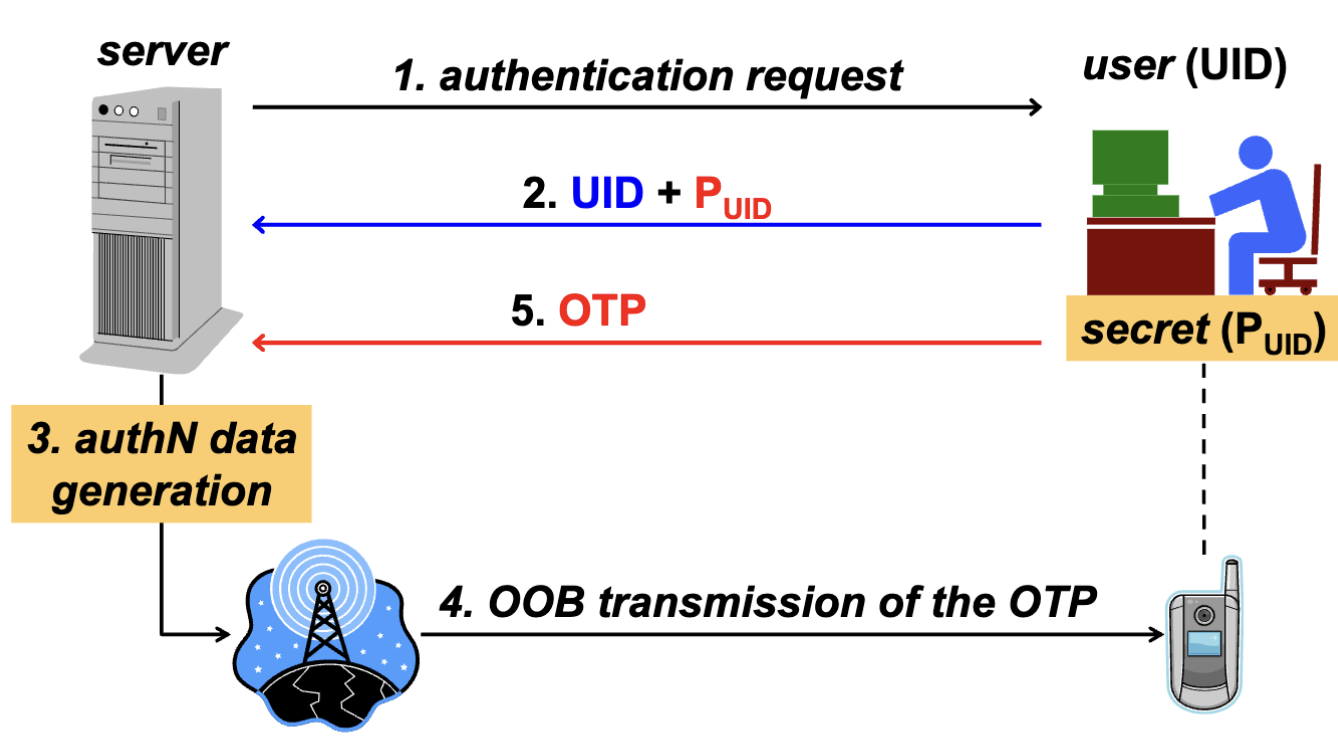
\includegraphics[width=\linewidth]{Images/Authentication/OOBotp.png}
        \caption{Out-of-Band One-Time Password}
    \end{figure}
\end{multicols}
\( \text{Assumptions: smart devices and network connectivity.} \)

\section{Two-/Multi-Factors Authentication}
\begin{center}
    2FA/MFA
\end{center}

\begin{itemize}
    \item Use more than one factor to authenticate the user: increased authentication strength and authenticator protection.
    \item PIN for authenticator protection:
    \begin{itemize}
        \item Transmitted along with OTP (secure channel).
        \item Used to compute the OTP itself.
        \item Used to unlock the authenticator (e.g., smart card), which can be very risky if:
        \begin{itemize}
            \item The lock mechanism is weak.
            \item There is no protection against multiple unlock attempts.
            \item Unlocking remains valid for a time window.
        \end{itemize}
    \end{itemize}
\end{itemize}
\section{Authentication of Human Beings}
How to authenticate a human being? The most common methods are:
\begin{itemize}
    \item CAPTCHA (Completely Automated Public Turing test to tell Computers and Humans Apart): A challenge-response test used to determine whether the user is human.
    \item Biometric techniques (e.g. fingerprint)
\end{itemize}

\subsection{Biometric Systems}
\begin{center}
    Identification, not only authentication.
\end{center}
Consists of a measure of a user's biological characteristic. The most common biometric techniques are: 
\begin{itemize}
    \item Fingerprint recognition.
    \item Facial recognition.
    \item Iris scanning.
    \item Voice recognition.
    \item Hand geometry.
    \item Retinal scanning.
\end{itemize}
Each technique can potentially be circumvented by an attacker. For example, fingerprint recognition can be bypassed by using a fake fingerprint. The security of a biometric system depends on the uniqueness of the biometric characteristic and the robustness of the system. Additionally, the biometric authentication is \textcolor{Red}{NOT REPLACEABLE}.

\subsection*{Biometric Systems - Issues}
Parameters related to the accuracy of biometric systems:
\begin{multicols}{2}
    \raggedcolumns

    \begin{itemize}
        \item FAR (False Acceptance Rate): The probability that the system incorrectly accepts an unauthorized user ("False Positive").
        \item FRR (False Rejection Rate): The probability that the system incorrectly rejects an authorized user("False Negative").
    \end{itemize}
\columnbreak

    \begin{figure}[H]
        \centering
        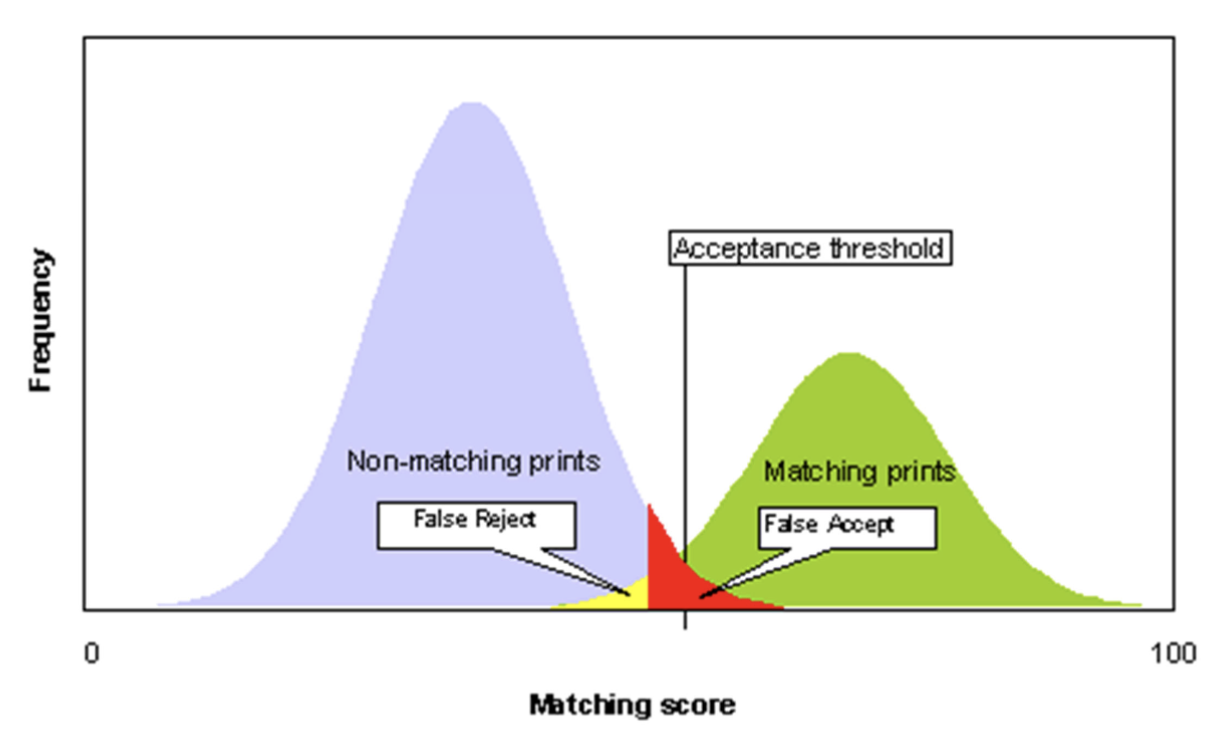
\includegraphics[width=\linewidth]{Images/Authentication/farrfrr.png}
        \caption{FAR and FRR}
    \end{figure}
\end{multicols}
FAR and FRR may be partly tuned, but they heavily depend on the cost of the system. Some variable biological characteristics are: finger wound, voice altered due to emotion or retinal blood pattern altered due to alcohol or drug.

\subsubsection*{Biometric Systems - Issues Analysis}

\begin{itemize}
    \item Psychological acceptance: Users may feel uncomfortable with biometric systems due to concerns about personal data collection, often referred to as the “Big Brother” syndrome. 
    \item Privacy: It's an identification (not just Authentication!!).
    \item Cannot be changed if copied, hence only useful to "locally" replace a PIN or a password.
    \item Lack of a standard API/SPI: high development costs and hevay dependence on single/few vendors.
\end{itemize}

\section{Kerberos}
\begin{center}
    Authentication System based on TTP (Trusted Third Party).
\end{center}



\begin{multicols}{2}
    \raggedcolumns

    \begin{center}
        Some key features:
    \end{center}
    \begin{itemize}
        \item Useful for non-HTTTP services.
        \item The TTP (Trusted Third Party) substitutes the Verifier.
        \item User's passwords are never transmitted but only used locally as (symmetric) cryptographic keys.
        \item Client authentication is compulsory (however, server authN is optional).
        \item Does not use Asymmetric Cryptography.
    \end{itemize}
\columnbreak

\begin{center}
    Definitions:
\end{center}
\begin{itemize}
    \item Realm (Kerberos Domain): A set of users and services that share the same Kerberos database.
    \item Credential: A set of information that proves the identity of a user.
    \[
        \text{user.instance@REALM}
    \]
    \item Ticket: A data structure used to authenticate a client to a server. It is encrypted with the symmetric key of the target server and is bound to the client’s IP address. The ticket is associated with only one credential.

\end{itemize}
\end{multicols}

\subsection*{Kerberos - Components}




\begin{multicols}{3}

    The Authentication Server 
    \hspace*{2.5cm}(AS)

\begin{itemize}
    \item The subscriber's credentials, used to derive a AS-Client session key.
    \item Each Ticket Granting Server, and their symmetric keys.
    \item Provides the client with a Ticket Granting Ticket (readable only by the TGS).
\end{itemize}
\columnbreak

The Ticket Granting Server 
\hspace*{2.5cm}(TGS)
\begin{itemize}
    \item The Application Servers IDs, and their symmetric keys.
    \item Provides the client with a Service Ticket (readable only by the server).
    \item Uses a symmetric session key, generated by the AS, to communicate with the client.
\end{itemize}
\columnbreak

The (Application) Server
\begin{itemize}
    \item Checks the Service Ticket and grants access to the client.
    \item Uses a symmetric session key, generated by the TGS, to communicate with the client.
\end{itemize}
\end{multicols}


\subsection{Kerberos - High-Level Overview}
\begin{center}
    A simplified view.
\end{center}
\[
    \boxed{\text{Client AuthN}} \rightarrow \boxed{\text{Service AuthN}} \rightarrow \boxed{\text{Service Access}}
\]
\dots \ using the entities:
\[
    \text{Authentication Server} \rightarrow \text{Ticket Granting Server} \rightarrow \text{(Application) Server}
\]
The three components act as a trusted third parties. Each entity has a symmetric key to communicate with the next one.

\begin{itemize}
    \item The client sends a request to the Authentication Server (AS) to authenticate his identity and specifying the Ticket Granting Server (TGS).
    \item The AS:
    \begin{itemize}
        \item Derives a symmetric key ("Session Key") $K_{\text{UID}}$ from the user's credential, in order to communicate with the TGS (Ticket Granting Server).
        \[\text{The Session Key } K_{\text{UID}} \text{ binds both Client and TGS}\]
        \item Issues a Ticket Granting Ticket (TGT) \underline{encrypted} with $K_{\text{TGS}}$.
        \[K_{\text{TGS}} \text{ is the AS-TGS symmetric key}\]
\end{itemize}
    \item The TGT is presented to the TGS (including an authenticator also, to prevent replay attacks) to request access to a specific service.
    \item The TGS:
    \begin{itemize}
        \item Issues a Service Ticket ("Access Token") $T_S$ \underline{encrypted} with $K_S$. 
        \[K_S \text{ is the TGS-Server symmetric key}\]
        \item The client presents the Service Ticket $T_S$ to the application server to access the desired service.
    \end{itemize} 
    \item If the Service Ticket $T_S$ is valid, the application server grants access.
\end{itemize}


\begin{multicols}{2}

    \begin{figure}[H]
        \centering
        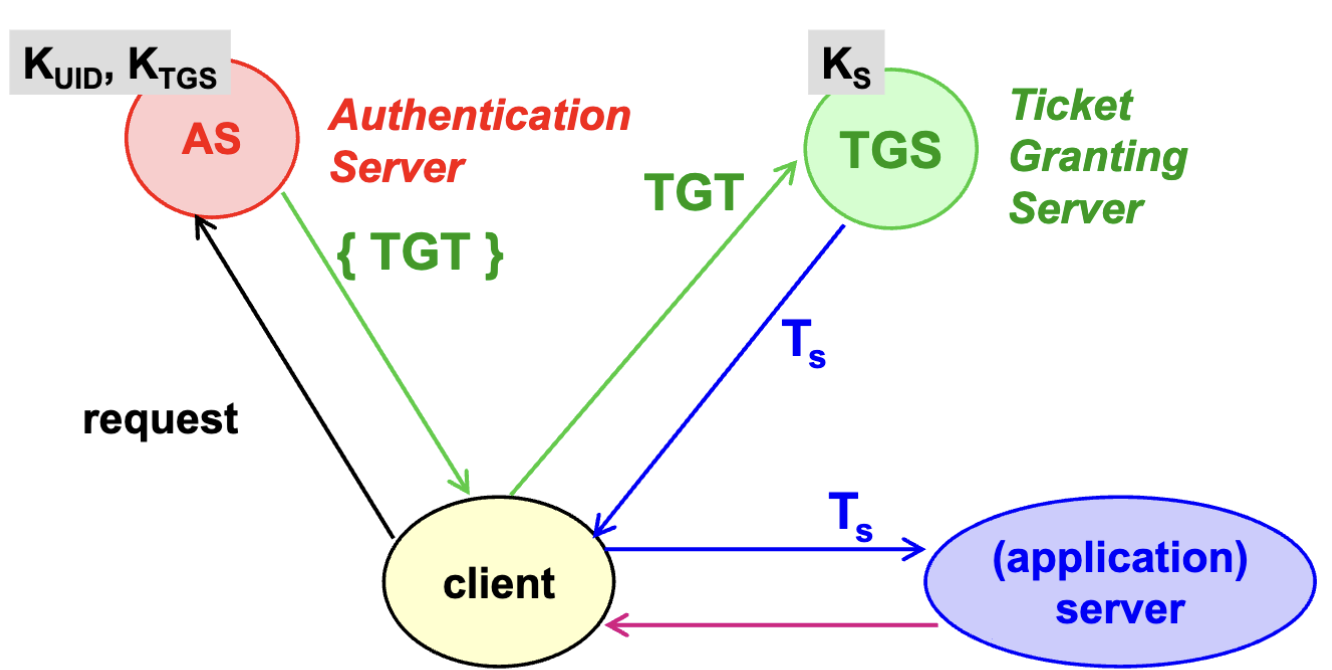
\includegraphics[width=\linewidth]{Images/Authentication/kerberosOverview.png}
        \caption{Kerberos Authentication Process Overview}
    \end{figure}
    \columnbreak

    \begin{figure}[H]
        \centering
        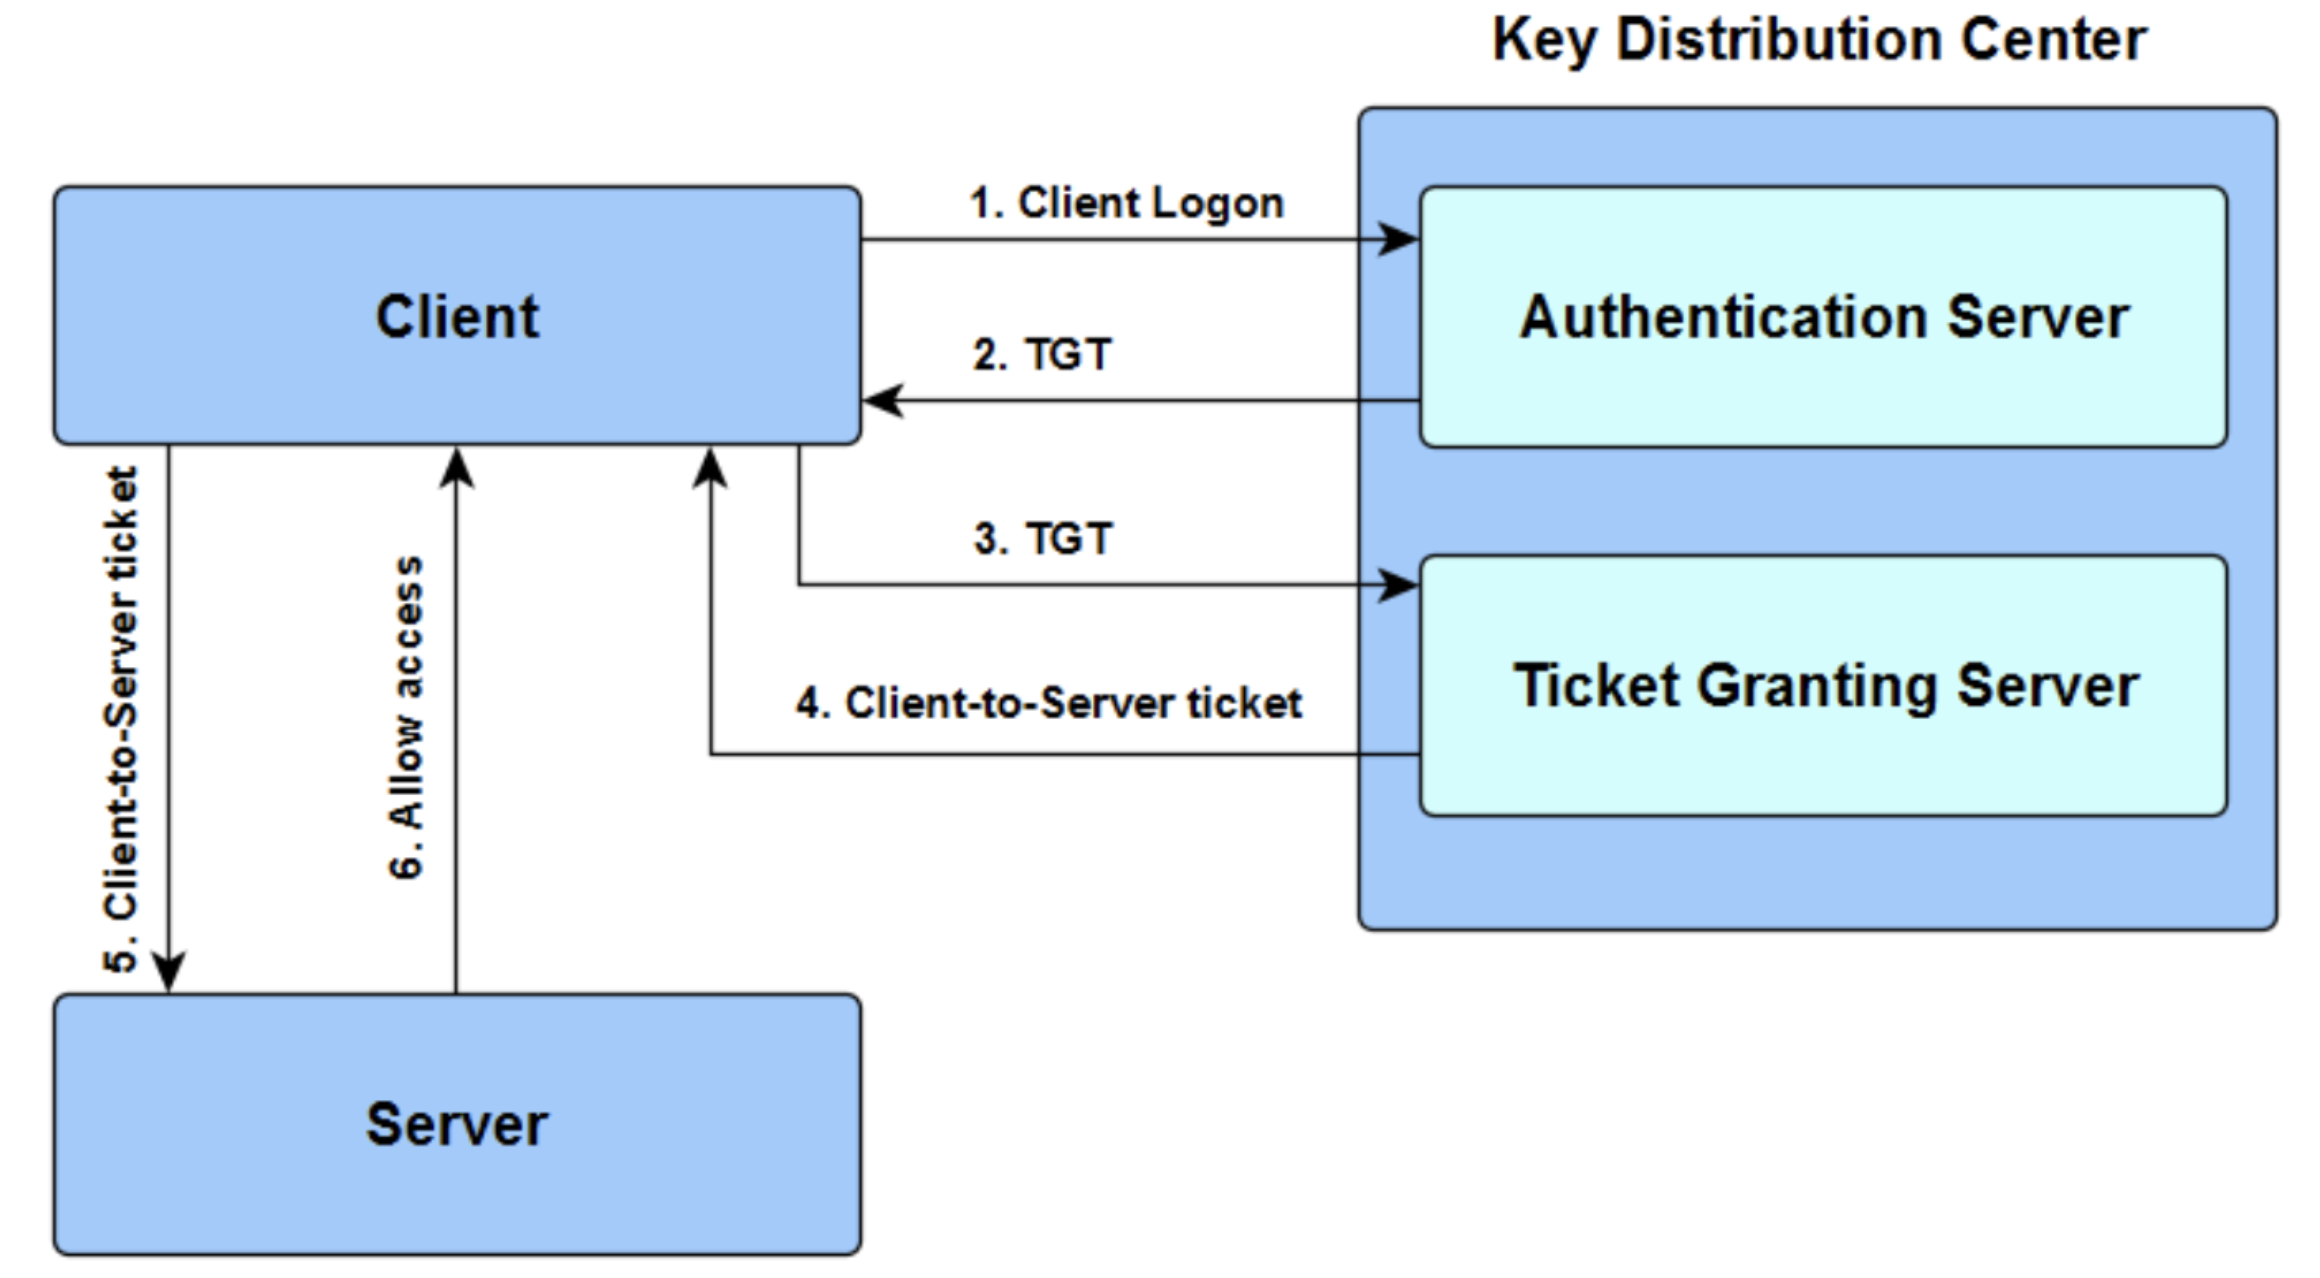
\includegraphics[width=\linewidth]{Images/Authentication/ker.png}
        \caption{Kerberos Authentication Process Overview}
    \end{figure}
    
\end{multicols}

\begin{tcolorbox}[colback=red!10!white, colframe=red!70!black, coltitle=white, title=Beware]
The servers must be very-well protected.
\end{tcolorbox}

\subsection*{Kerberos - Data Formats (v4)}
The data structures used in Kerberos v4 are:
\begin{figure}[H]
    \centering
    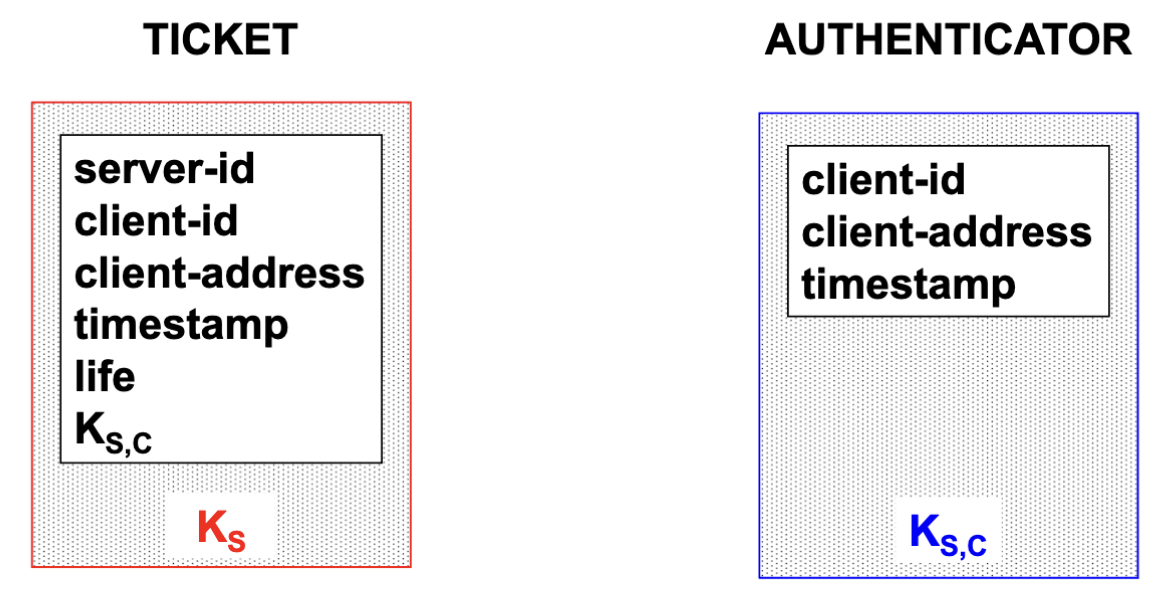
\includegraphics[width=0.5\linewidth]{Images/Authentication/kerDataFormats.png}
    \caption{Kerberos Data Formats (v4)}
\end{figure}

\subsection*{Kerberos - TGT request}
\begin{center}
    Ticket Granting Ticket request process.
\end{center}
Intro:
The client requests a Ticket Granting Ticket (TGT) from the Authentication Server (AS).
\begin{itemize}
    \item The client sends:
    \begin{enumerate}
        \item The client's ID $C$.
        \item The specific TGS.
    \end{enumerate} 
    \item The AS responds by generating and sending to the Client:
    \begin{enumerate}
        \item A session key $K_{C,TGS}$ for the client and the TGS.
        \item A Ticket Granting Ticket (TGT)  $T_{\text{C,TGS}}$ \underline{encrypted} with the specific TGS's secret key $K_{\text{TGS}}$, so only the TGS can verify it.
        
        \begin{center}
            Both the session key and the encrypted TGT are sent to the client \underline{encrypted} with the client's secret key $K_{\text{C}}$.
        \end{center}
    \end{enumerate}
\end{itemize}
\begin{figure}[H]
    \centering
    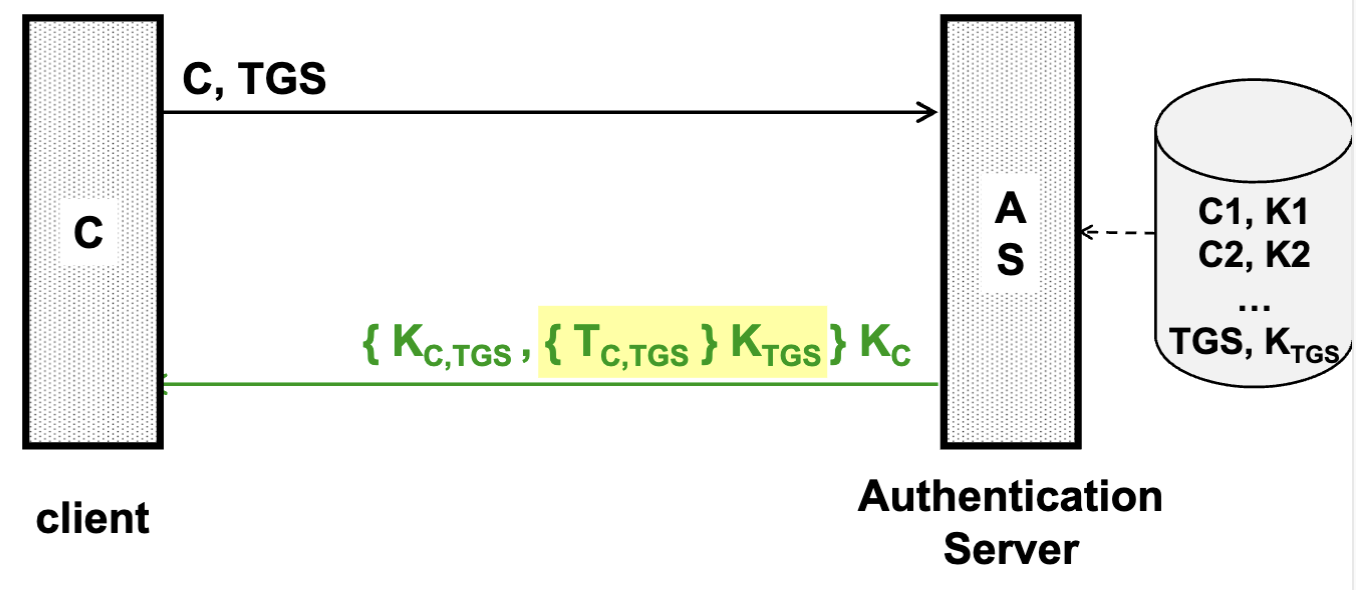
\includegraphics[width=0.5\linewidth]{Images/Authentication/kerreq.png}
    \caption{Kerberos TGT Request}
\end{figure}

\subsection*{Kerberos - Service Ticket request}
Intro: The client requests a Service Ticket from the Ticket Granting Server (TGS) to access a specific service.

\begin{itemize}
    \item The Client sends:
    \begin{enumerate}
        \item The specific server $S$.
        \item The Ticket-Granting Ticket $T_{\text{C,TGS}}$, which was encrypted with the TGS's secret key $K_{\text{TGS}}$.
        \item \textcolor{Blue}{In addition...} The Client authenticator $A_C$ (preventing replay attacks), \underline{encrypted} with the Client-TGS session key forged by the Authentication Server.
    \end{enumerate} 
    \item The TGS responds by generating and sending to the Client:
    \begin{enumerate}
        \item The Service Ticket $T_{\text{C,S}}$ \underline{encrypted} with the Server's secret key $K_{\text{S}}$.
        \item The Client-Server session key $K_{\text{C,S}}$.
        
        \begin{center}
            Both the Service Ticket and the session key are \underline{encrypted} with the Client-TGS session key.

        \end{center}
    \end{enumerate}
\end{itemize}

\begin{figure}[H]
    \centering
    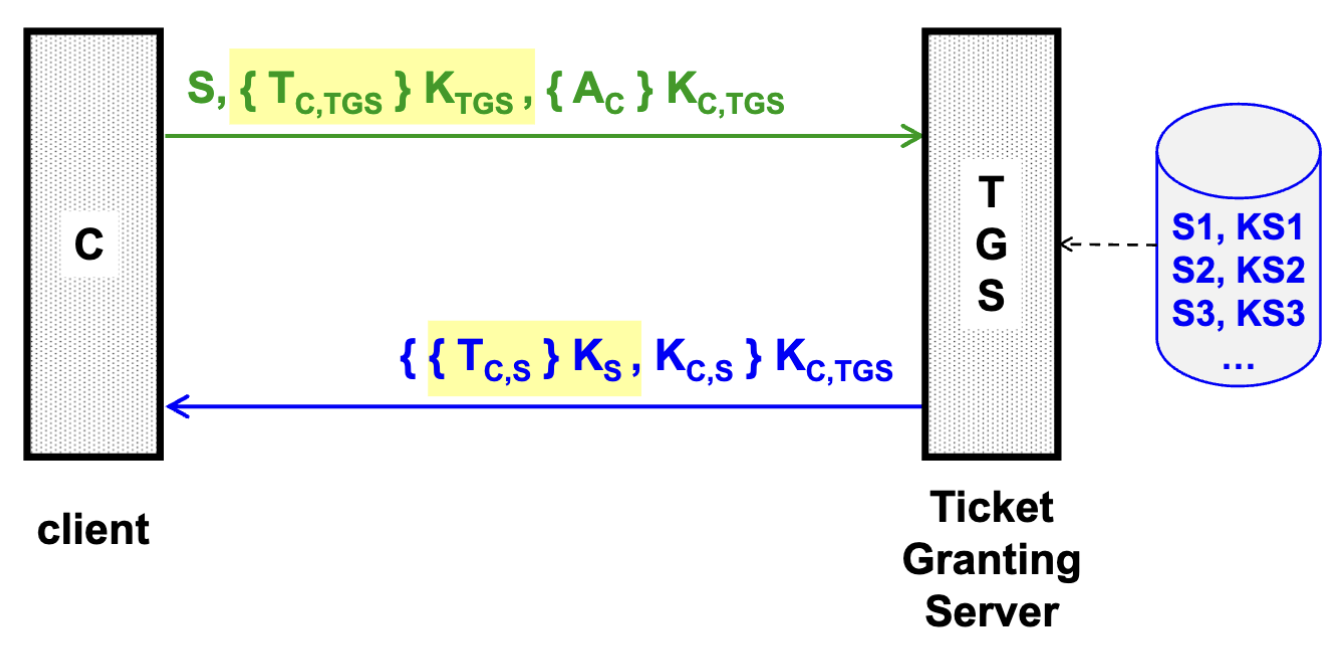
\includegraphics[width=0.5\linewidth]{Images/Authentication/kerticketreq.png}
    \caption{Kerberos Ticket Request}
\end{figure}

\subsection*{Kerberos - Service Ticket use}

Intro: The Client tries to use the Service Ticket to access the desired service.
\begin{itemize}
    \item The Client sends:
    \begin{enumerate}
        \item The Service Ticket $T_{\text{C,S}}$ encrypted with the Server's secret key $K_{\text{S}}$.
        \item The Authenticator $A_C$ (preventing replay attacks), \underline{encrypted} with the Client-Server session key $K_{\text{C,S}}$.
    \end{enumerate}
    \item The Server responds by:
    \begin{itemize}
        \item Sending the specific time ($timestamp(A_C)$) at which the Authenticator $A_C$ was created, encrypted with the Client-Server session key $K_{\text{C,S}}$.
    \end{itemize}
\end{itemize}

\begin{figure}[H]
    \centering
    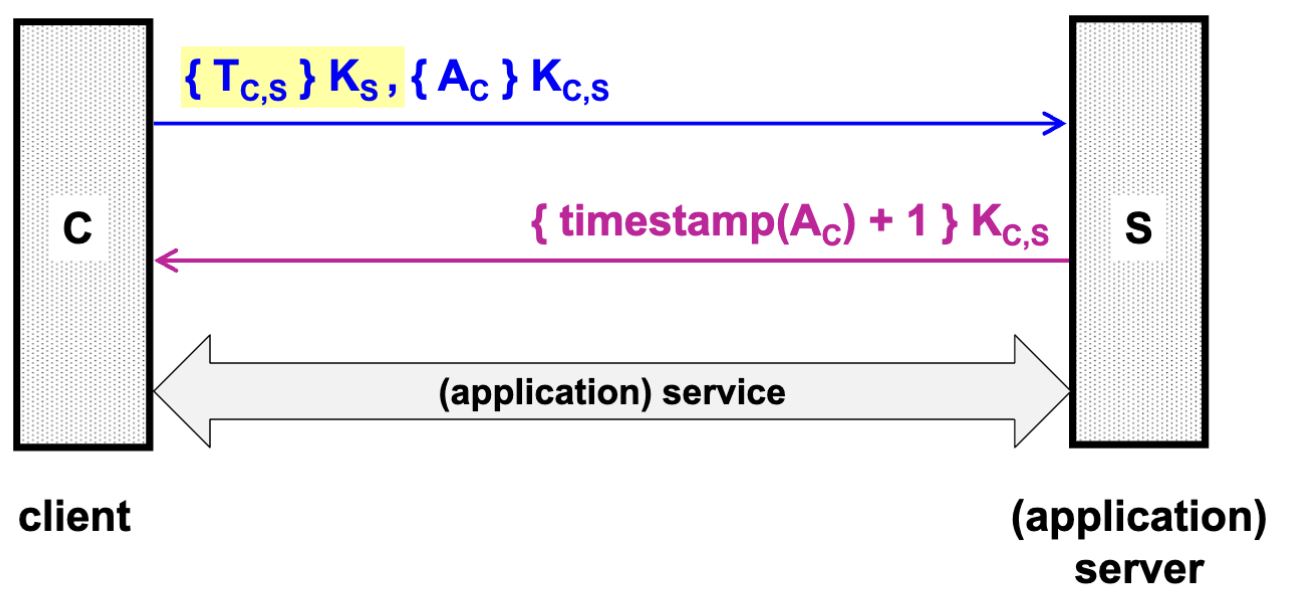
\includegraphics[width=0.5\linewidth]{Images/Authentication/kerticketuse.png}
    \caption{Kerberos Ticket Use}
\end{figure}

\subsection*{Kerberos - Versions and Usage}
\begin{itemize}
    \item Kerberos v4: The first version.
    \item Kerberos v5.
    \begin{itemize}
        \item Not only DES encryption.
        \item Extended ticket lifetime.
        \item Inter realm authentication.
        \item Forwardable tickets.
        \item Extendable ticket.
    \end{itemize}
    \item Single login to all Kerberized services.
    \begin{itemize}
        \item K-POP (Post Office Protocol), K-LPD (Line Printer Daemon), K-FTP (File Transfer Protocol), K-TELNET.
        \item Services in a Windows domain (Microsoft has adopted Kerberos\footnote{A specific Microsoft version with proprietary data structures.} since Windows 2000).    \end{itemize}
\end{itemize}

\subsection{Kerberos - V5}
\begin{center}
    RFC-4120
\end{center}
Key features:
\begin{itemize}
    \item Algorithm flexibility:
    \begin{itemize}
        \item Client and servers may support different algorithms.
        \item Originally used DES-CRC32, then 3DES, RC4, AES, Camellia and MD4, MD5.
    \end{itemize}
    \item Pre-authentication to prevent password enumeration or dictionary attacks on the TGT.
    \item Support for asymmetric crypto (only for \texttt{AS\_REQ})
\end{itemize}

\subsubsection*{Kerberos v5 - Public Key Cryptography for Initial Authentication in Kerberos.}
\begin{center}
    TGT request with PKINIT.
    \\ Asymmetric encryption used only for the initial authentication with the Authentication Server.
    \\The AS knows the client ID and its public key.
\end{center}
Intro: The client tries to authenticate itself to the Authentication Server (AS) using public key cryptography.
\begin{itemize}
    \item The Client sends:
    \begin{itemize}
        \item The client's ID.
        \item The specific TGS.
    \end{itemize}
    \item The AS responds by sending:
    \begin{itemize}
        \item A session key $K_{C,TGS}$ for the client and the TGS.
        \item A Ticket Granting Ticket (TGT)  $T_{\text{C,TGS}}$ \underline{encrypted} with the specific TGS's secret key $K_{\text{TGS}}$, so only the TGS can verify it.
        \begin{center}
            Both the session key and the encrypted TGT are sent to the client \underline{encrypted} with the client's public key $\text{C.PK}$.
        \end{center}
        
    \end{itemize}
\end{itemize}
\begin{figure}[H]
    \centering
    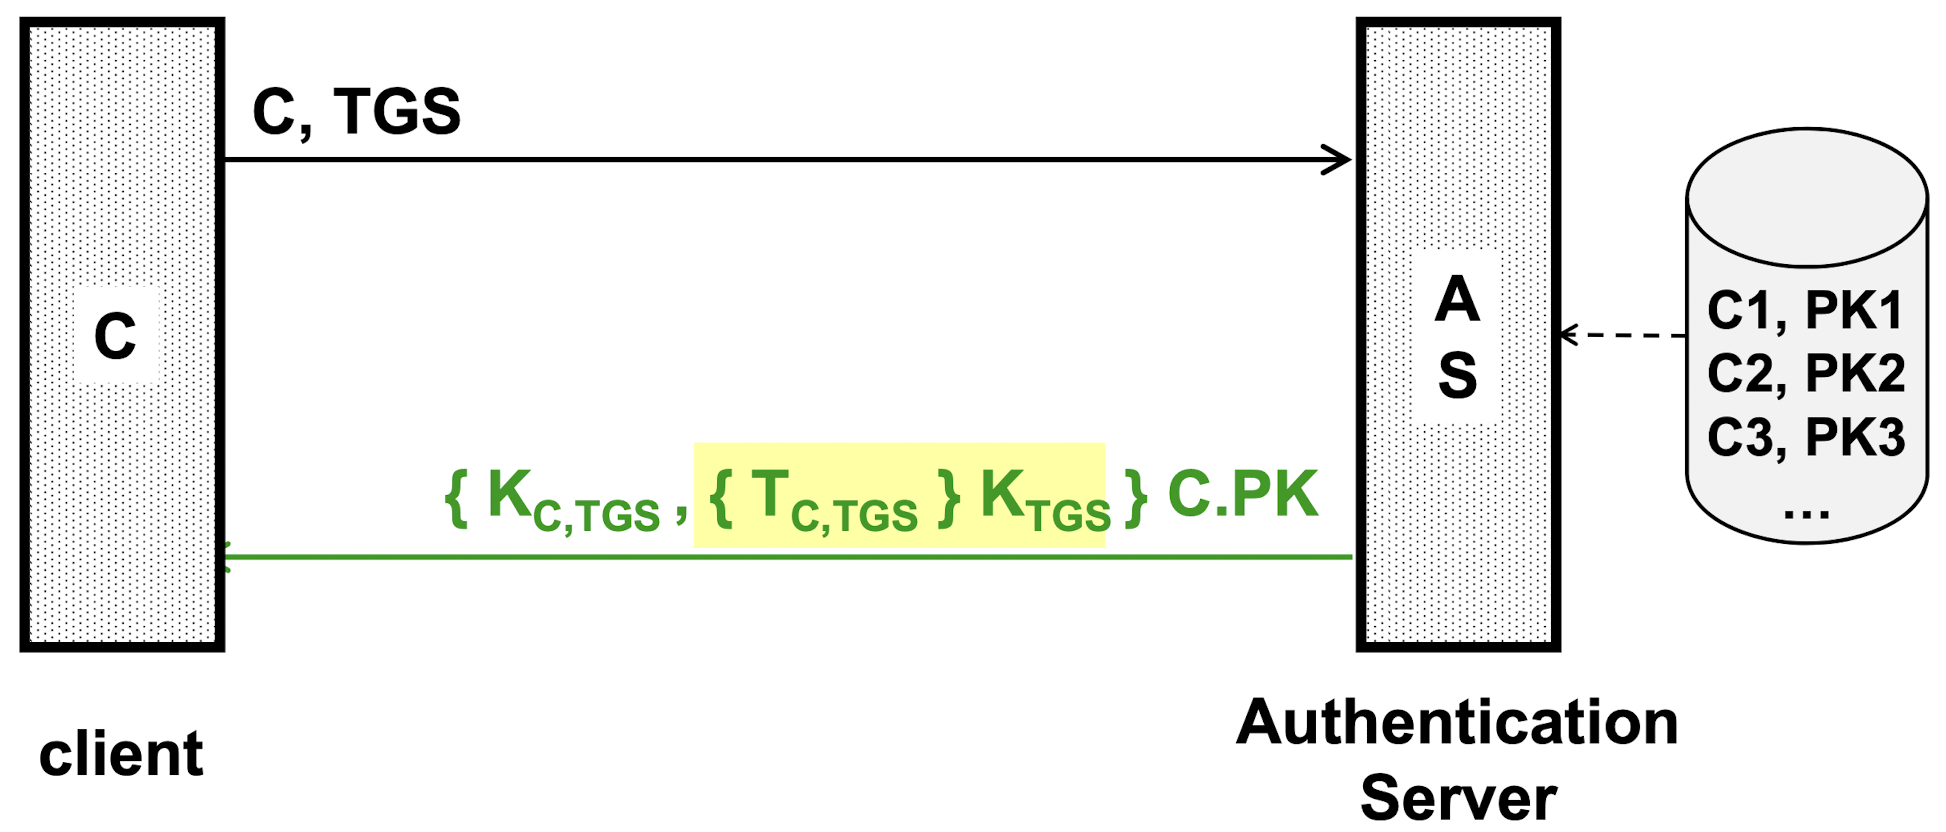
\includegraphics[width=0.5\linewidth]{Images/Authentication/kerv5.png}
    \caption{Kerberos v5 - PKINIT}
\end{figure}

\section{Single Sign-On}
\begin{center}
    SSO
\end{center}
The user has a single credential to authenticate himself and access any service in the system.
Two main approaches:
\begin{itemize}
    \item \textbf{Fictitious SSO:}
    \begin{itemize}
        \item The client is used for automatic password synchronization/management (commonly referred to as a "password wallet").
        \item Specific to certain applications only.
    \end{itemize}
    \item \textbf{Integral SSO:}
    \begin{itemize}
        \item Utilizes multi-application authentication techniques (e.g., asymmetric Credential Request Authentication (CRA), Kerberos).
        \item Supports multi-domain SSO (e.g., through SAML tokens, which generalize Kerberos tickets).
    \end{itemize}
\end{itemize}
\section{Open Authentication Initiative (OATH)}
\begin{center}
    For Authentication Interoperability.
\end{center}


\begin{multicols}{2}

    Scopes:
    \begin{itemize}
        \item Ensuring interoperability of authentication systems based on OTPs and symmetric/asymmetric challenge-response mechanisms.  
        \item Development of standards for client-server protocols and data formats on the client side.
    \end{itemize}
\columnbreak

\begin{figure}[H]
    \centering
    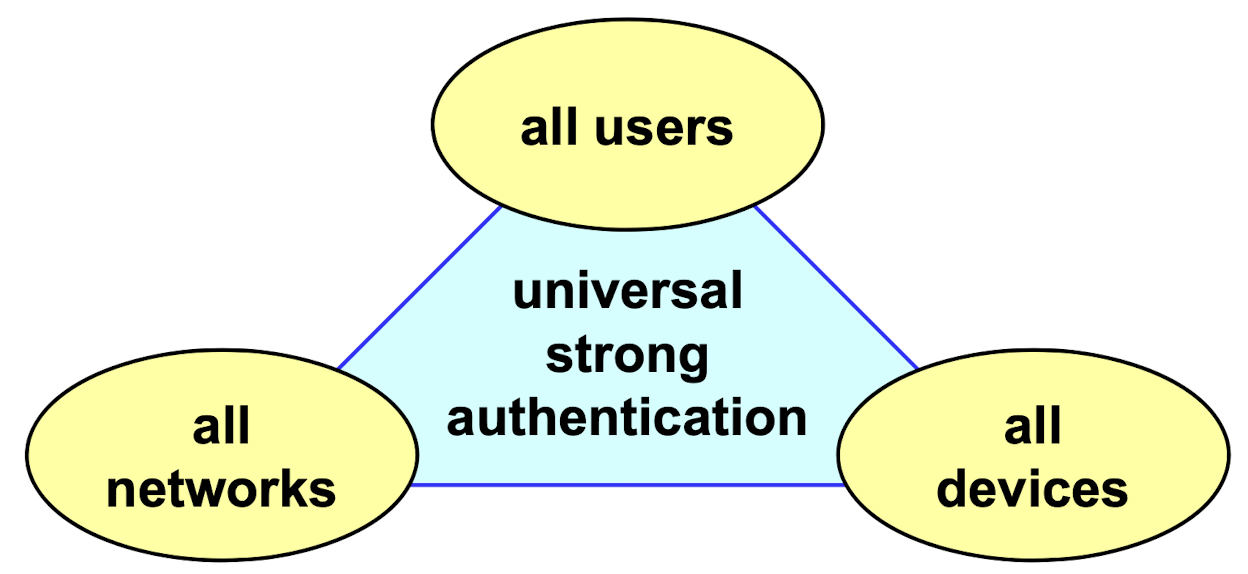
\includegraphics[width=\linewidth]{Images/Authentication/oath.png}
    \caption{Open Authentication Initiative}
\end{figure}

\end{multicols}

\subsection*{OATH - Specifications}
\begin{itemize}
    \item HOTP (HMAC-based One-Time Password - RFC-4226).
    \item TOTP (Time-based One-Time Password - RFC-6238).
    \item OATH challenge- response protocol (OCRA, RFC-6287).
    \item Portable Symmetric Key Container (PSKC, RFC-6030): XML-based key container for transporting symmetric keys and key-related meta-data.
    \item Dynamic Symmetric Key Provisioning Protocol (DSKPP, RFC-6063): Client-Server protocol for provisioning symmetric keys to a crypto-engine by a key-provisioning server.
\end{itemize}

\subsection{OATH - HMAC-based One-Time Password}
\begin{center}
    Method for generating event-based OTPs (One-Time Passwords).
\end{center}
Key features:
\begin{itemize}
    \item HOTP works by incrementing the counter  C  for each event, making it event-based rather than time-based.
    \item HOTP can be used as an Out-of-Band OTP mechanism.
\end{itemize}

\noindent HOTP Generation Formula:
\[HOTP(K,C)=sel\big(\text{HMAC-h}(K,C)\big)\quad \&\quad \text{0x7FFFFFFF}\]
\begin{itemize}
    \item K: Shared secret key.
    \item C: Monotonic positive integer counter.
    \item h: Cryptographic hash function (default: SHA-1).
    \item HMAC-h: HMAC function based on the hash function h.
    \item sel: Function to select a subset of the hash output (default: 4 bytes).
\end{itemize}
The mask 0x7FFFFFFF is used to set MSB (Most Significant Bit) to 0 (avoiding issues when treating the result as a signed integer.).

\hspace*{1cm}

\noindent To generate $N$ digits access code (HOTP code) (suggested: 6-8):
\[\text{HOTP-code} = HOTP (K, C) \mod \, 10^N\]

\subsection{OATH: Time-based One-Time Password}
Key features:
Works as HOTP but the counter $C$ is the number of intervals $TS$ elapsed since a fixed origin $T_0$.
    \[
        C= \dfrac{T-T_0}{TS}
    \]
\noindent Defaults:
\begin{itemize}
    \item $T_0$ = Unix epoch (00:00:00 UTC on 1 January 1970).
    \item $T$ = Unix time (seconds elapsed since $T_0$).
    \item For example, $TS$ = 30 seconds is equivalent to $C=\lfloor\dfrac{T}{30}\rfloor$.
    \item h: SHA1 (but MAY use SHA256 or SHA512).
    \item N: 6 digits.
\end{itemize}
\subsection{Google Authenticator}
Supports HOTP and TOTP with the following assumptions:
\begin{itemize}
    \item K: base\-32 encoded shared secret.
    \item C: uint\_64 counter.
    \item sel(X), selection function for 4 bytes of X:
    \begin{itemize}
        \item offset=4 least significant bits of X.
        \item return X[offset:offset+3].
    \end{itemize}
    \item $TS$: 30 seconds.
    \item $N$: 6 digits.
\end{itemize}
If the generated code contains less than 6 digits then it's left padded with zeroes (e.g. $123 > 000123$).
\section{Fast Identity Online}
\begin{center}
    FIDO - based on asymmetric cryptography.
\end{center}
\begin{itemize}
    \item Is the industry standard of the FIDO Alliance, for:
    \begin{itemize}
        \item Biometric authentication (often referred as "passwordless user experience").
        \item Second-factor authentication (often referred as "$2^{nd}$ factor user experience").
    \end{itemize}
    \item Is based on personal devices capable of \underline{asymmetric cryptography}.
\end{itemize}
Components:
\begin{itemize}
    \item UAF (Universal Authentication Framework): Biometric authentication.
    \item U2F (Universal Second Factor): Second-factor authentication.
    \item ASM (Authenticator Specific Model): Security model for the authenticator.
\end{itemize}
FIDO is available for major services (Google, Dropbox. GitHub, Twitter) and also for the cloud (GCP, AWS, Azure).

\subsection*{FIDO - Login Process}
Secure authentication flow for a user logging into a website, typically with a FIDO-compliant authentication device.
\begin{multicols}{2}

    \begin{enumerate}
        \item The user initiates the login process on a website (SITE.COM) by entering their username (e.g., “BOB”).

        A login challenge is generated and sent to the user’s device or authentication system.
        \item The user approves the login request (e.g., by tapping a button, scanning a fingerprint, or entering a PIN).
        \item Upon user approval, the FIDO device selects the private key associated with the website (SITE.COM) and uses it to sign the login challenge.
        
        The signed login response is sent back to the website.
        \item The website verifies the signature using the user’s public key, which was securely stored during registration.
    \end{enumerate}
    \columnbreak

    \begin{figure}[H]
        \centering
        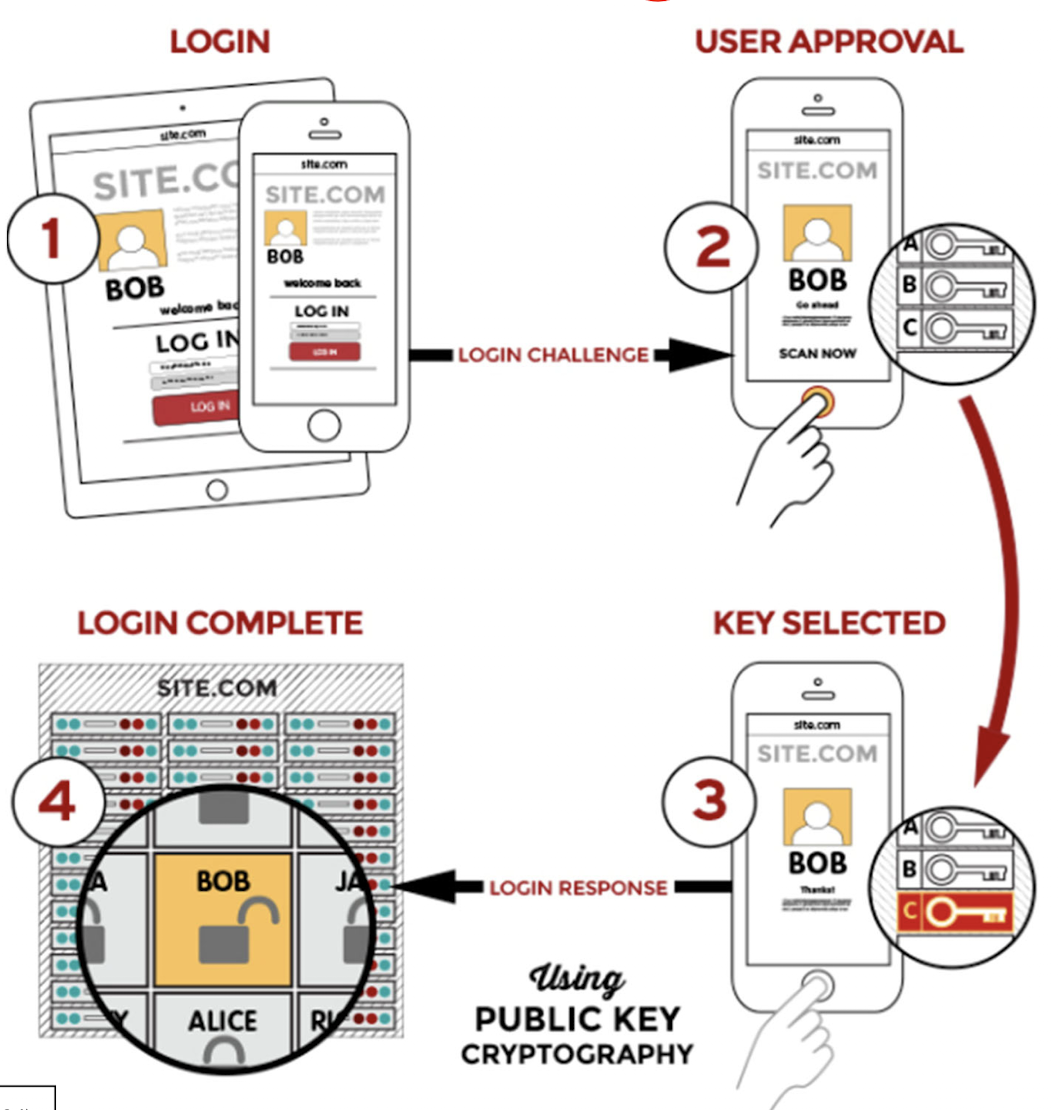
\includegraphics[width=\linewidth]{Images/Authentication/fidolog.png}
        \caption{FIDO Login process}
    \end{figure}
    
\end{multicols}
If the signature is valid, the website completes the login process, granting access to “BOB.”
\clearpage
\subsection*{FIDO - Universal Second Factor Registration Process}
The flow involves securely generating and exchanging public/private key pairs to enable strong, passwordless, or two-factor authentication.
\begin{multicols}{2}

    \begin{enumerate}
        \item The user agent (browser or app) begins the registration process. The website forwards this request to its FIDO U2F backend.
        \item A registration request and a hash (cryptographic challenge) are sent to the FIDO U2F device.
        \item The U2F device performs the following actions: generates a key pair (public key and private key) and generates a key handle, which is a reference to the private key stored securely within the device.
        \item The FIDO U2F device sends a registration response back to the user agent. Contains: the public key (generated by the device) and the key handle (used to identify the key pair securely).
        \item The FIDO U2F backend (installed on the RP) verifies the registration response and stores the public key and key handle.
    \end{enumerate}
\columnbreak

    \begin{figure}[H]
        \centering
        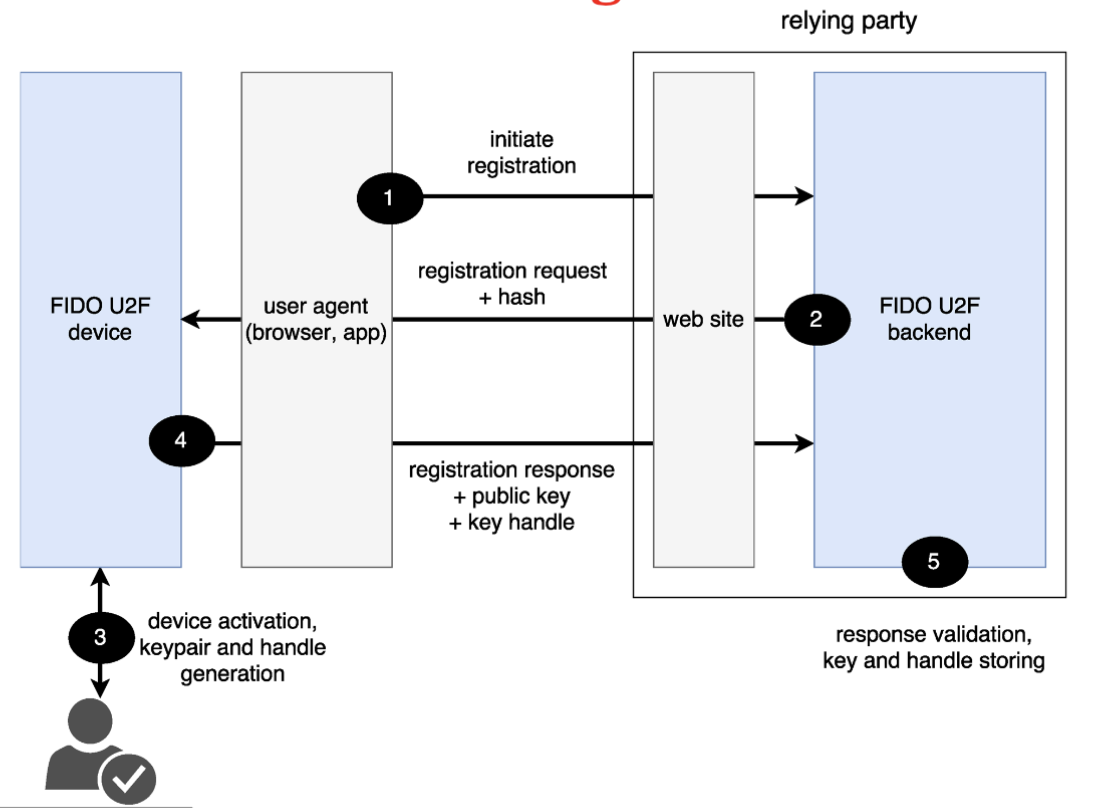
\includegraphics[width=\linewidth]{Images/Authentication/fidoreg.png}
        \caption{FIDO Universal Second Factor registration process}
    \end{figure}
\end{multicols}

\subsection*{FIDO - Universal Second Factor Authentication}

\begin{multicols}{2}

\begin{enumerate}
    \item The user agent (browser or app) sends a username/password to the website (relying party).
    \item The FIDO U2F backend generates a challenge and retrieves the key handle (stored during the registration process). Both are sent to the FIDO U2F device.
    \item The U2F device chooses the correct private key (based on the key handle) and signs the challenge. 
    \item The signed challenge is sent back to the user agent, who forwards it to the FIDO U2F backend.
    \item The FIDO U2F backend verifies the challenge solution.
\end{enumerate}

\columnbreak

    \begin{figure}[H]
        \centering
        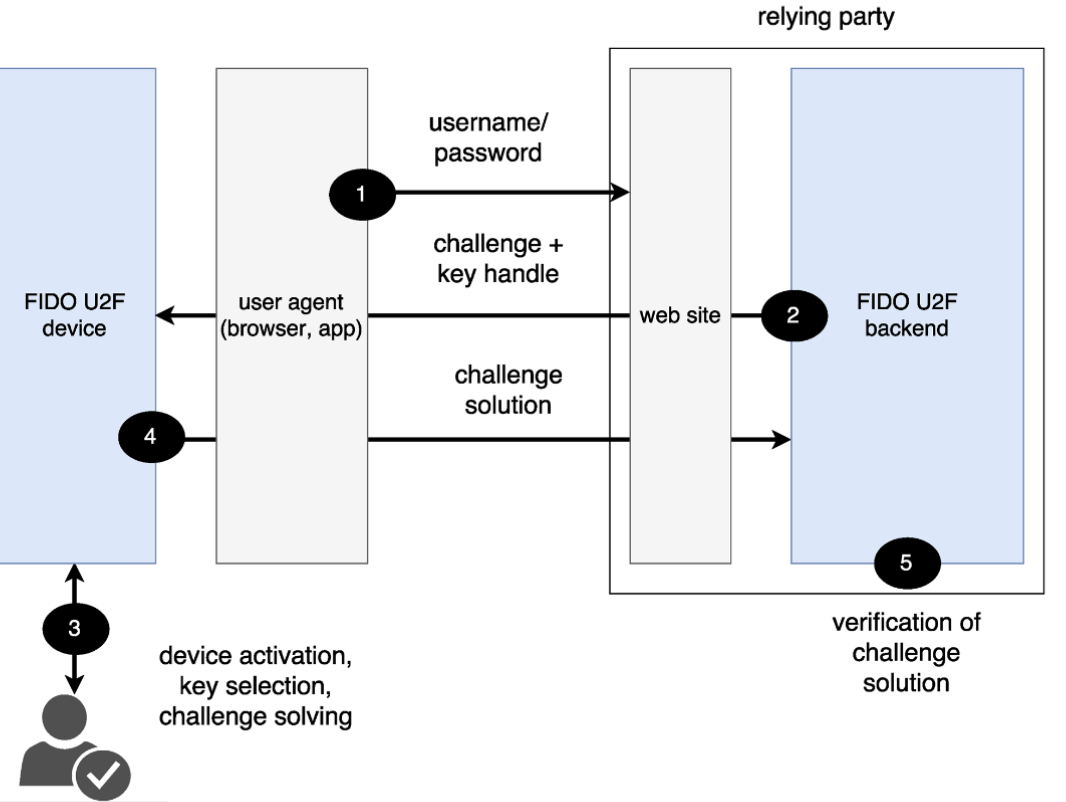
\includegraphics[width=\linewidth]{Images/Authentication/fidoauthn.png}
        \caption{FIDO Universal Second Factor Authentication}
    \end{figure}
\end{multicols}

If the signature matches, the authentication is successful.

\subsection*{FIDO - Other Characteristics}
\begin{itemize}
    \item \textbf{Biometric techniques}: Local authentication methods (e.g., fingerprint, facial recognition) used to unlock and enable the use of \textbf{FIDO keys} stored securely on the user device. Biometric data remains on the device and is not transmitted.
    
    \item \textbf{Secure transactions}: Digital signatures are applied to transaction-specific texts (in addition to responding to the server's challenge) to ensure transaction integrity and prevent replay attacks or similar threats.
    
    \item \textbf{FIDO backend (or server)}: The FIDO server validates user authentication by verifying challenge responses or transaction signatures using the corresponding \textbf{public keys}. It enables secure and standardized FIDO-based authentication on an application server.
    
    \item \textbf{FIDO client}: A client-side component (e.g., browser, application, or user agent) that interacts with the FIDO device to create, manage, and use \textbf{FIDO credentials} stored on the user device for authentication.
\end{itemize}

\subsection*{FIDO - Security Considerations}
\begin{itemize}
    \item \textbf{Strong authentication}: Achieved using asymmetric cryptography (public/private key pairs).
    \item \textbf{No third parties involved}: The authentication process occurs directly between the user and the relying party.
    \item \textbf{No secrets on the server side}: The server does not store any sensitive secrets, only public keys.
    \item \textbf{Biometric data}: If biometrics are used, they never leave the user’s device and remain local.
    \item \textbf{No phishing}: Authentication responses cannot be reused because they are signatures over multiple data points, including the Relying Party's identity.
    \item \textbf{Unlinkability}: A new key pair is generated for every registration. This ensures no linkability between different services used by the same user or different accounts owned by the same user.
    \item \textbf{No key storage limits}: Private keys are not stored in the authenticator but are dynamically recomputed as needed based on an internal secret and the Relying Party's identity.
\end{itemize}

\subsection*{FIDO 2.0}
Components for authentication:
\begin{itemize}
    \item CTAP (Client to Authenticator Protocol): Enables communication between clients (e.g., browsers) and authenticators (e.g., hardware tokens or devices).
    \item The platform (bound, internal) authenticators: Built-in authenticators within devices (e.g., smartphones, laptops). They rely on cryptographic elements to securely store and use asymmetric keys (public-private key pairs).
\end{itemize}

Attestation ensures the legitimacy of an authenticator by verifying its integrity and manufacturer origin. Here are listed some types of attestations:
\begin{itemize}
    \item Packed Attestation: Authenticators with limited resources, like a Secure Element (SE).
    \item TPM Attestation: Uses a Trusted Platform Module (TPM), a secure cryptographic processor for authentication.
    \item Android Key Attestation: Uses Android’s secure key storage (introduced in Android Nougat) for authentication.
    \item Android SafetyNet Attestation: Uses the SafetyNet API to verify the security status of Android devices.
    \item Future Extension for IoT: FIDO 2.0 is being extended to include authentication for IoT devices to improve security in the IoT ecosystem.
\end{itemize}

\subsection*{FIDO 2.0 - How It Works}
\begin{enumerate}
    \item The RP app triggers an authentication request through the web authN JS API.
    \item The browser and platform coordinate with the (platform) authenticator or an external (roaming) authenticator (via CTAP).
    \item The authenticator generates a cryptographic signature using private keys.
    \item The Relying Party server validates the signature with help from the FIDO server, completing the authentication.
\end{enumerate}

\begin{figure}[H]
    \centering
    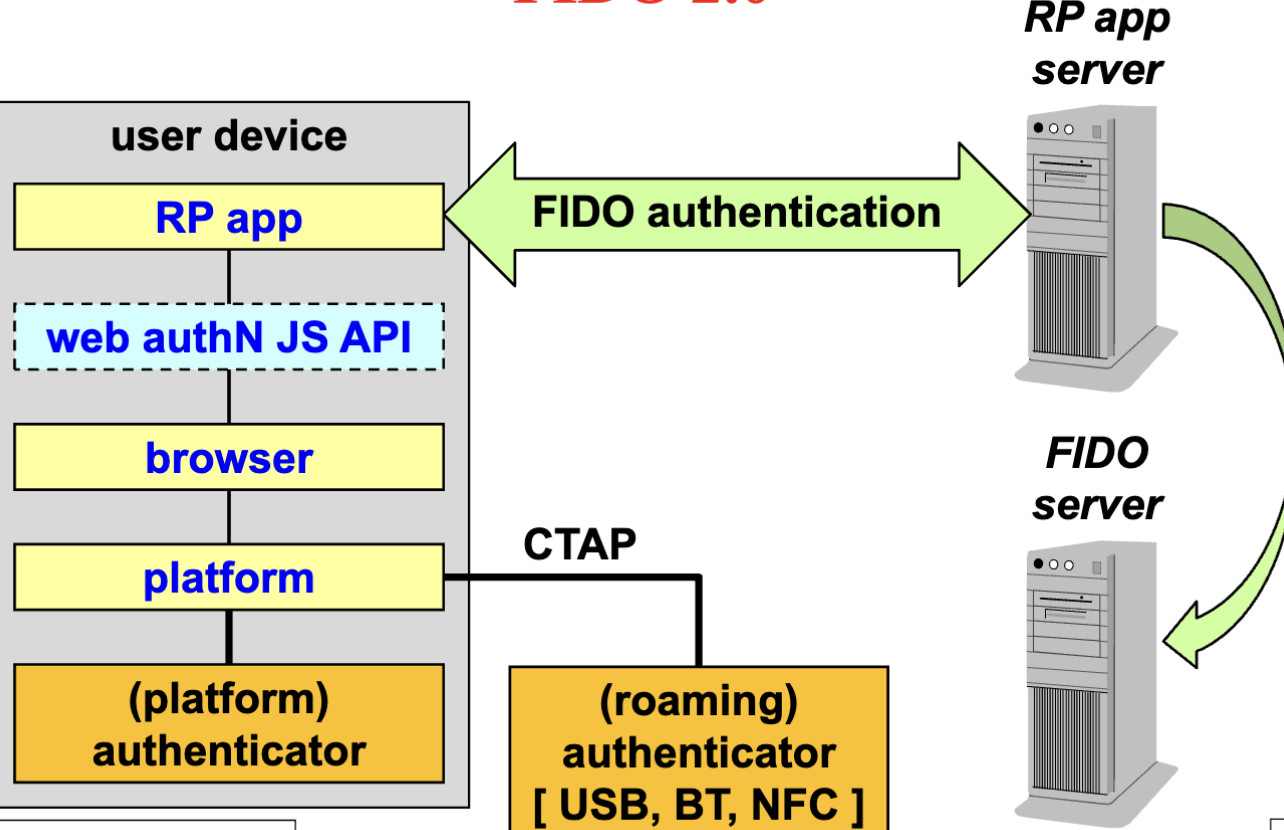
\includegraphics[width=0.5\linewidth]{Images/Authentication/fido2.png}
    \caption{FIDO 2.0 - How It Works}
\end{figure}